\textbackslash{}chapter\{Fundamental Concepts\}
\textbackslash{}label\{ch:1\}

This book is about Lagrangians and Hamiltonians. To state it more formally,
this book is about the variational approach to analytical mechanics. You may
not have been exposed to the calculus of variations, or may have forgotten what
you once knew about it, so I am not assuming that you know what I mean by,
``the variational approach to analytical mechanics.'' But I think that by the time
you have worked through the first two chapters, you will have a good grasp of
the concept.
We being with a review of introductory concepts and an overview of background material. Some of the concepts presented in this chapter will be familiar from your introductory and intermediate mechanics courses. However, you
will also encounter several new concepts that will be useful in developing an
understanding of advanced analytical mechanics.
\section*{1.1  Kinematics}

A particle is a material body having mass but no spatial extent. Geometrically,
it is a point. The position of a particle is usually specified by the vector r from
the origin of a coordinate system to the particle. We can assume the coordinate system is inertial and for the sake of familiarity you may suppose the
\begin{figure}[h]
\centering
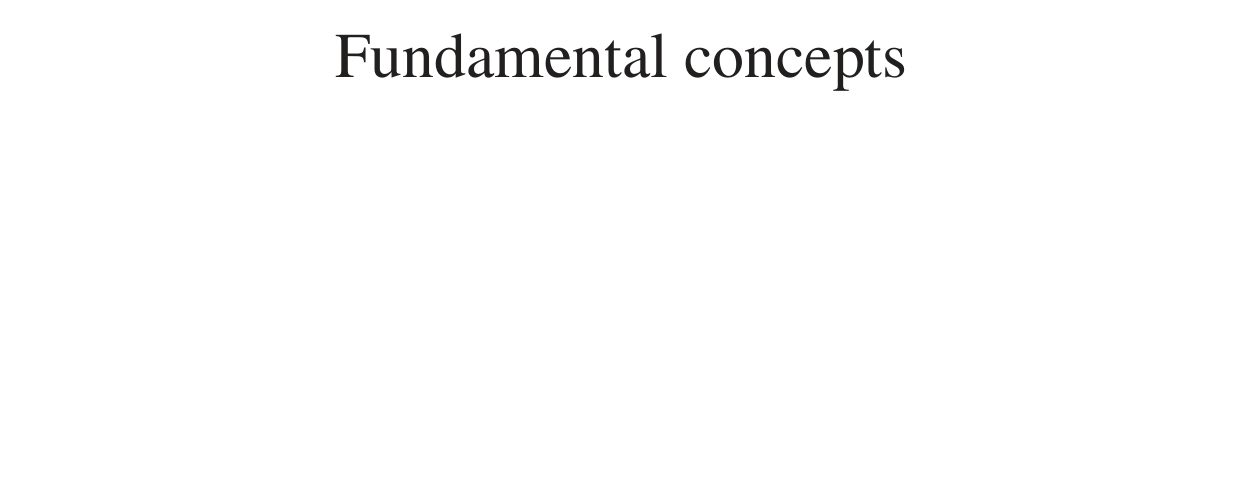
\includegraphics[width=0.55\linewidth]{../Figures/fig_1_1.png}
\caption{Figure 1.1}
\end{figure}

The velocity of a particle is defined as the time rate of change of its position
and the acceleration of a particle is defined as the time rate of change of its
velocity. That is,
v =dr
dt = $\textbackslash{}dot r$,
(1.1)

y
z
r
The position of a particle is specified by the vector r.
and
a =dv
dt = $\textbackslash{}ddot r$.
(1.2)
The equation for a as a function of r, $\textbackslash{}dot r$, and t is called the equation of
motion. The equation of motion is a second-order differential equation whose
solution gives the position as a function of time, r = r(t). The equation of
motion can be solved numerically for any reasonable expression for the acceleration and can be solved analytically for a few expressions for the acceleration. You may be surprised to hear that the only general technique for solving
the equation of motion is the procedure embodied in the Hamilton--Jacobi
equation that we will consider in Chapter 6. All of the solutions you have been
exposed to previously are special cases involving very simple accelerations.
Typical problems, familiar to you from your introductory physics course,
involve falling bodies or the motion of a projectile. You will recall that the projectile problem is two-dimensional because the motion takes place in a plane.
It is usually described in Cartesian coordinates.
Another important example of two-dimensional motion is that of a particle
moving in a circular or elliptic path, such as a planet orbiting the Sun. Since
the motion is planar, the position of the body can be specified by two coordinates. These are frequently the plane polar coordinates (r, \textbackslash{}theta ) whose relation to
Cartesian coordinates is given by the transformation equations
x = r cos \textbackslash{}theta ,
y = r sin \textbackslash{}theta .
This is an example of a point transformation in which a point in the xy plane
is mapped to a point in the r\textbackslash{}theta  plane.

1.2
Generalized coordinates
You will recall that in polar coordinates the acceleration vector can be
resolved into a radial component and an azimuthal component
a = $\textbackslash{}ddot r$ = ar \textbackslash{}hat\{r\}+a\textbackslash{}theta  ˆ\textbackslash{}theta .
(1.3)
\begin{exercise}
Exercise 1.1 A particle is given an impulse which imparts to it a velocity v0. It then undergoes an acceleration given by a = -bv, where b
is a constant and v is the velocity. Obtain expressions for v = v(t)
and x = x(t). (This is a one-dimensional problem.) Answer: x(t) =
x0 + (v0/b)

1 -e-bt
.
\end{exercise}

\begin{exercise}
Exercise 1.2 Assume the acceleration of a body of mass m is given by
a = -(k/m)x. (a) Write the equation of motion. (b) Solve the equation of
motion. (c) Determine the values of the arbitrary constants (or constants
of integration) if the object is released from rest at x = A. (The motion
is called ``simple harmonic.'') Answer (c): x = A sin
\textbackslash{}sqrtk/mt + \textbackslash{}pi /2

=
A cos \textbackslash{}sqrtk/mt.
\end{exercise}

\begin{exercise}
Exercise 1.3 In plane polar coordinates, the position is given by r = r\textbackslash{}hat\{r\}.
Obtain expressions for the velocity and acceleration in terms of r, \textbackslash{}theta , \textbackslash{}hat\{r\}, ˆ\textbackslash{}theta .
(Hint: Express \textbackslash{}hat\{r\} and ˆ\textbackslash{}theta  in terms of \textbackslash{}hat\{i\} and \textbackslash{}hat\{j\}.) Answer: a = ($\textbackslash{}ddot r$-r $\textbackslash{}dot\textbackslash{}$theta 2)\textbackslash{}hat\{r\}+(r $\textbackslash{}ddot \textbackslash{}theta$  +
2$\textbackslash{}dot r$ $\textbackslash{}dot\textbackslash{}$theta )ˆ\textbackslash{}theta .
\end{exercise}

\section*{1.2  Generalized coordinates}

In the preceding section we stated that the position of the particle was given
by the vector r. We assumed an inertial Cartesian coordinate system in which
the components of r were (x, y, z). Of course, there are many other ways we
could have specified the position of the particle. Some ways that immediately
come to mind are to give the components of the vector r in cylindrical (\textbackslash{}rho , \textbackslash{}phi , z)
or in spherical coordinates (r, \textbackslash{}theta , \textbackslash{}phi ). Obviously, a particular problem can be
formulated in terms of many different sets of coordinates.
In three-dimensional space we need three coordinates to specify the position
of a single particle. For a system consisting of two particles, we need six coordinates. A system of N particles requires 3N coordinates. In Cartesian coordinates, the positions of two particles might be described by the set of numbers
(x1, y1, z1, x2, y2, z2). For N particles the positions of all the particles are
(x1, y1, z1, x2, y2, z2, . . . , xN, yN, zN).

As you know, some problems are more easily solved in one coordinate system
and some are more easily solved in another. To avoid being specific about the
coordinate system we are using, we shall denote the coordinates by qi and
the corresponding velocities by $\textbackslash{}dot q$i. We call qi the ``generalized coordinates.''
Of course, for any particular problem you will chose an appropriate set of
coordinates; in one problem you might use spherical coordinates in which case
as i ranges from 1 to 3, the coordinates qi take on the values r, \textbackslash{}theta , \textbackslash{}phi , whereas
in another problem you might use cylindrical coordinates and qi = \textbackslash{}rho , \textbackslash{}phi , z.
To convert from Cartesian coordinates to generalized coordinates, you need to
know the transformation equations, that is, you need to know the relations
q1 = q1(x1, y1, z1, x2, y2, . . . , zN, t)
(1.4)
q2 = q2(x1, y1, z1, x2, y2, . . . , zN, t)
...
q3N = q3N(x1, y1, z1, x2, y2, . . . , zN, t).
The inverse relations are also called transformation equations. For a system of
N particles we have
x1 = x1(q1, q2, . . . , q3N, t)
(1.5)
y1 = y2(q1, q2, . . . , q3N, t)
...
zN = zN(q1, q2, . . . , q3N, t).
It is often convenient to denote all the Cartesian coordinates by the letter x.
Thus, for a single particle, (x, y, z) is written (x1, x2, x3) and, for N particles,
(x1, y1, . . . , zN) is expressed as (x1, . . . , xn), where n = 3N.
We usually assume that given the transformation equations from the qs to the
xs, we can carry out the inverse transformation from the xs to the qs, but this
is not always possible. The inverse transformation is possible if the Jacobian
determinant of Equations (1.4) is not zero. That is,
\textbackslash{}partial (q1, q2, . . . , qn)
\textbackslash{}partial (x1, x2, . . . , xn) =

\textbackslash{}partial q1/\textbackslash{}partial x1
\textbackslash{}partial q1/\textbackslash{}partial x2
\textbackslash{}cdot  \textbackslash{}cdot  \textbackslash{}cdot
\textbackslash{}partial q1/\textbackslash{}partial xn
...
\textbackslash{}partial qn/\textbackslash{}partial x1
\textbackslash{}partial qn/\textbackslash{}partial x2
\textbackslash{}cdot  \textbackslash{}cdot  \textbackslash{}cdot
\textbackslash{}partial qn/\textbackslash{}partial xn
̸
= 0.
The generalized coordinates are usually assumed to be linearly independent,
and thus form a minimal set of coordinates to describe a problem. For example,
the position of a particle on the surface of a sphere of radius a can be described
in terms of two angles (such as the longitude and latitude). These two angles

1.3
Generalized velocity
form a minimal set of linearly independent coordinates. However, we could
also describe the position of the particle in terms of the three Cartesian coordinates, x, y, z. Clearly, this is not a minimal set. The reason is that the Cartesian
coordinates are not all independent, being related by x2 + y2 + z2 = a2. Note
that given x and y, the coordinate z is determined. Such a relationship is called
a ``constraint.'' We find that each equation of constraint reduces by one the
number of independent coordinates.
Although the Cartesian coordinates have the property of being components
of a vector, this is not necessarily true of the generalized coordinates. Thus,
in our example of a particle on a sphere, two angles were an appropriate set
of generalized coordinates, but they are not components of a vector. In fact,
generalized coordinates need not even be coordinates in the usual sense of
the word. We shall see later that in some cases the generalized coordinates
can be components of the momentum or even quantities that have no physical
interpretation.
When you are actually solving a problem, you will use Cartesian coordinates or cylindrical coordinates, or whatever coordinate system is most convenient for the particular problem. But for theoretical work one nearly always
expresses the problem in terms of the generalized coordinates (q1, . . . , qn).
As you will see, the concept of generalized coordinates is much more than a
notational device.
\begin{exercise}
Exercise 1.4 Obtain the transformation equations for Cartesian coordinates to spherical coordinates. Evaluate the Jacobian determinant for
this transformation. Show how the volume elements in the two coordinate systems are related to the Jacobian determinant. Answer: d\textbackslash{}tau  =
r2 sin \textbackslash{}theta drd\textbackslash{}theta d\textbackslash{}phi .
\end{exercise}

\section*{1.3  Generalized velocity}

As mentioned, the position of a particle at a particular point in space can be
specified either in terms of Cartesian coordinates ($\textbackslash{}xi$) or in terms of generalized
coordinates (qi). These are related to one another through a transformation
equation:
$\textbackslash{}xi$ = $\textbackslash{}xi$(q1, q2, q3, t).
Note that $\textbackslash{}xi$, which is one of the three Cartesian coordinates of a specific particle, depends (in general) on all the generalized coordinates.

We now determine the components of velocity in terms of generalized coordinates.
The velocity of a particle in the $\textbackslash{}xi$ direction is vi and by definition
vi \textbackslash{}equiv dxi
dt .
But $\textbackslash{}xi$ is a function of the qs, so using the chain rule of differentiation we have
vi =

k=1
\textbackslash{}partial $\textbackslash{}xi$
\textbackslash{}partial qk
dqk
dt + \textbackslash{}partial $\textbackslash{}xi$
\textbackslash{}partial t =

k
\textbackslash{}partial $\textbackslash{}xi$
\textbackslash{}partial qk
$\textbackslash{}dot q$k + \textbackslash{}partial $\textbackslash{}xi$
\textbackslash{}partial t .
(1.6)
We now obtain a very useful relation involving the partial derivative of vi with
respect to $\textbackslash{}dot q$j. Since a mixed second-order partial derivative does not depend
on the order in which the derivatives are taken, we can write
\textbackslash{}partial
\textbackslash{}partial $\textbackslash{}dot q$j
\textbackslash{}partial $\textbackslash{}xi$
\textbackslash{}partial t = \textbackslash{}partial
\textbackslash{}partial t
\textbackslash{}partial $\textbackslash{}xi$
\textbackslash{}partial $\textbackslash{}dot q$j
.
But \textbackslash{}partial $\textbackslash{}xi$
\textbackslash{}partial $\textbackslash{}dot q$j = 0 because x does not depend on the generalized velocity $\textbackslash{}dot q$. Let us
take the partial derivative of vi with respect to $\textbackslash{}dot q$j using Equation (1.6). This
yields
\textbackslash{}partial vi
\textbackslash{}partial $\textbackslash{}dot q$j
=
\textbackslash{}partial
\textbackslash{}partial $\textbackslash{}dot q$j

k
\textbackslash{}partial $\textbackslash{}xi$
\textbackslash{}partial qk
$\textbackslash{}dot q$k +
\textbackslash{}partial
\textbackslash{}partial $\textbackslash{}dot q$j
\textbackslash{}partial $\textbackslash{}xi$
\textbackslash{}partial t
=
\textbackslash{}partial
\textbackslash{}partial $\textbackslash{}dot q$j

k
\textbackslash{}partial $\textbackslash{}xi$
\textbackslash{}partial qk
$\textbackslash{}dot q$k + 0
=

k
\textbackslash{}partial
\textbackslash{}partial $\textbackslash{}dot q$j
\textbackslash{}partial $\textbackslash{}xi$
\textbackslash{}partial qk

$\textbackslash{}dot q$k +

k
\textbackslash{}partial $\textbackslash{}xi$
\textbackslash{}partial qk
\textbackslash{}partial $\textbackslash{}dot q$k
\textbackslash{}partial $\textbackslash{}dot q$j
= 0 +

k
\textbackslash{}partial $\textbackslash{}xi$
\textbackslash{}partial qk
\textbackslash{}delta ij
= \textbackslash{}partial $\textbackslash{}xi$
\textbackslash{}partial qj
.
Thus, we conclude that
\textbackslash{}partial vi
\textbackslash{}partial $\textbackslash{}dot q$j
= \textbackslash{}partial $\textbackslash{}xi$
\textbackslash{}partial qj
.
(1.7)
This simple relationship comes in very handy in many derivations concerning generalized coordinates. Fortunately, it is easy to remember because
it states that the Cartesian velocity is related to the generalized velocity in
the same way as the Cartesian coordinate is related to the generalized
coordinate.

1.4
Constraints
\section*{1.4  Constraints}

Every physical system has a particular number of degrees of freedom. The
number of degrees of freedom is the number of independent coordinates needed
to completely specify the position of every part of the system. To describe the
position of a free particle one must specify the values of three coordinates (say,
x, y and z). Thus a free particle has three degrees of freedom. For a system
of two free particles you need to specify the positions of both particles. Each
particle has three degrees of freedom, so the system as a whole has six degrees
of freedom. In general a mechanical system consisting of N free particles will
have 3N degrees of freedom.
When a system is acted upon by forces of constraint, it is often possible to
reduce the number of coordinates required to describe the motion. Thus, for
example, the motion of a particle on a table can be described in terms of x and
y, the constraint being that the z coordinate (defined to be perpendicular to the
table) is given by z = constant. The motion of a particle on the surface of a
sphere can be described in terms of two angles, and the constraint itself can
be expressed by r = constant. Each constraint reduces by one the number of
degrees of freedom.
In many problems the system is constrained in some way. Examples are
a marble rolling on the surface of a table or a bead sliding along a wire. In
these problems the particle is not completely free. There are forces acting on
it which restrict its motion. If a hockey puck is sliding on smooth ice, the
gravitational force is acting downward and the normal force is acting upward.
If the puck leaves the surface of the ice, the normal force ceases to act and the
gravitational force quickly brings it back down to the surface. At the surface,
the normal force prevents the puck from continuing to move downward in the
vertical direction. The force exerted by the surface on the particle is called a
force of constraint.
If a system of N particles is acted upon by k constraints, then the number of
generalized coordinates needed to describe the motion is 3N -k. (The number of Cartesian coordinates is always 3N, but the number of (independent)
generalized coordinates is 3N -k.)
A constraint is a relationship between the coordinates. For example, if a
particle is constrained to the surface of the paraboloid formed by rotating
a parabola about the z axis, then the coordinates of the particle are related
by z -x2/a -y2/b = 0. Similarly, a particle constrained to the surface
of a sphere has coordinates that are related by x2 + y2 + z2 -
a2 = 0.

If the equation of constraint (the relationship between the coordinates) can
be expressed in the form
f (q1, q2, . . . , qn, t) = 0,
(1.8)
then the constraint is called holonomic.1
The key elements in the definition of a holonomic constraint are: (1) the
equals sign and (2) it is a relation involving the coordinates. For example, a possible constraint is that a particle is always outside of a sphere of
radius a. This constraint could be expressed as r \textbackslash{}geq a. This is not a holonomic constraint. Sometimes a constraint involves not just coordinates but
also velocities or differentials of the coordinates. Such constraints are also not
holonomic.
As an example of a non-holonomic constraint consider a marble rolling on
a perfectly rough table. The marble requires five coordinates to completely
describe its position and orientation, two linear coordinates to give its position
on the table top and three angle coordinates to describe its orientation. If the
table top is perfectly smooth, the marble can slip and there is no relationship
between the linear and angular coordinates. If, however, the table top is rough
there are relations (constraints) between the angle coordinates and the linear
coordinates. These constraints will have the general form dr = ad\textbackslash{}theta , which
is a relation between differentials. If such differential expressions can be integrated, then the constraint becomes a relation between coordinates, and it is
holonomic. But, in general, rolling on the surface of a plane does not lead to
integrable relations. That is, in general, the rolling constraint is not holonomic
because the rolling constraint is a relationship between differentials. The equation of constraint does not involve only coordinates. (But rolling in a straight
line is integrable and hence holonomic.)
A holonomic constraint is an equation of the form of (1.8) relating the generalized coordinates, and it can be used to express one coordinate in terms of
the others, thus reducing the number of coordinates required to describe the
motion.
\begin{exercise}
Exercise 1.5 A bead slides on a wire that is moving through space in a
complicated way. Is the constraint holonomic? Is it scleronomous?
1 A constraint that does not contain the time explicitly is called scleronomous. Thus
x2 + y2 + z2 -a2 = 0 is both holonomic and scleronomous.

1.5
Virtual displacements
\end{exercise}

\begin{exercise}
Exercise 1.6 Draw a picture showing that a marble can roll on a tabletop
and return to its initial position with a different orientation, but that there
is a one-to-one relation between angle and position for rolling in a straight
line.
\end{exercise}

\begin{exercise}
Exercise 1.7 Express the constraint for a particle moving on the surface
of an ellipsoid.
\end{exercise}

\begin{exercise}
Exercise 1.8 Consider a diatomic molecule. Assume the atoms are point
masses. The molecule can rotate and it can vibrate along the line joining
the atoms. How many rotation axes does it have? (We do not include operations in which the final state cannot be distinguished from the initial state.)
How many degrees of freedom does the molecule have? (Answer: 6.)
\end{exercise}

\begin{exercise}
Exercise 1.9 At room temperature the vibrational degrees of freedom of
O2 are ``frozen out.'' How many degrees of freedom does the oxygen
molecule have at room temperature? (Answer: 5.)
\end{exercise}

\section*{1.5  Virtual displacements}

A virtual displacement, \textbackslash{}delta $\textbackslash{}xi$, is defined as an infinitesimal, instantaneous displacement of the coordinate $\textbackslash{}xi$, consistent with any constraints acting on the
system.
To appreciate the difference between an ordinary displacement dxi and a
virtual displacement \textbackslash{}delta $\textbackslash{}xi$, consider the transformation equations
$\textbackslash{}xi$ = $\textbackslash{}xi$(q1, q2, . . . , qn, t)
i = 1, 2, . . . , 3N.
Taking the differential of the transformation equations we obtain
dxi = \textbackslash{}partial $\textbackslash{}xi$
\textbackslash{}partial q1
dq1 + \textbackslash{}partial $\textbackslash{}xi$
\textbackslash{}partial q2
dq2 + \textbackslash{}cdot  \textbackslash{}cdot  \textbackslash{}cdot  + \textbackslash{}partial $\textbackslash{}xi$
\textbackslash{}partial qn
dqn + \textbackslash{}partial $\textbackslash{}xi$
\textbackslash{}partial t dt
=
n

\textbackslash{}alpha =1
\textbackslash{}partial $\textbackslash{}xi$
\textbackslash{}partial q\textbackslash{}alpha
dq\textbackslash{}alpha  + \textbackslash{}partial $\textbackslash{}xi$
\textbackslash{}partial t dt.
But for a virtual displacement \textbackslash{}delta $\textbackslash{}xi$, time is frozen, so
\textbackslash{}delta $\textbackslash{}xi$ =
n

\textbackslash{}alpha =1
\textbackslash{}partial $\textbackslash{}xi$
\textbackslash{}partial q\textbackslash{}alpha
dq\textbackslash{}alpha .
(1.9)

\section*{1.6  Virtual work and generalized force}

Suppose a system is subjected to a number of applied forces. Let Fi be the force
component along $\textbackslash{}xi$. (Thus, for a two-particle system, F5 would be the force in
the y direction acting on particle 2.) Allowing all the Cartesian coordinates to
undergo virtual displacements \textbackslash{}delta $\textbackslash{}xi$, the virtual work performed by the applied
forces will be
\textbackslash{}delta W =
3N

i=1
Fi\textbackslash{}delta $\textbackslash{}xi$.
Substituting for \textbackslash{}delta $\textbackslash{}xi$ from Equation (1.9)
\textbackslash{}delta W =
3N

i=1
Fi
3N

\textbackslash{}alpha =1
\textbackslash{}partial $\textbackslash{}xi$
\textbackslash{}partial q\textbackslash{}alpha
\textbackslash{}delta q\textbackslash{}alpha

.
Interchanging the order of the summations
\textbackslash{}delta W =
3N

\textbackslash{}alpha =1
3N

i=1
Fi
\textbackslash{}partial $\textbackslash{}xi$
\textbackslash{}partial q\textbackslash{}alpha

\textbackslash{}delta q\textbackslash{}alpha .
Harkening back to the elementary concept of ``work equals force times distance'' we define the generalized force as
Q\textbackslash{}alpha  =
3N

i=1
Fi
\textbackslash{}partial $\textbackslash{}xi$
\textbackslash{}partial q\textbackslash{}alpha
.
(1.10)
Then the virtual work can be expressed as
\textbackslash{}delta W =
3N

\textbackslash{}alpha =1
Q\textbackslash{}alpha \textbackslash{}delta q\textbackslash{}alpha .
Equation (1.10) is the definition of generalized force.
\begin{example}
Example 1.1 Show that the principle of virtual work (\textbackslash{}delta W = 0 in equilibrium)
implies that the sum of the torques acting on the body must be zero.
Solution 1.1 Select an axis of rotation in an arbitrary direction . Let the
body rotate about  through an infinitesimal angle ϵ. The virtual displacement
of a point Pi located at Ri relative to the axis is given by
\textbackslash{}delta Ri = ϵ \textbackslash{}times  Ri.
The work done by a force Fi acting on Pi is
\textbackslash{}delta Wi = Fi \textbackslash{}cdot  \textbackslash{}delta Ri = Fi \textbackslash{}cdot  (ϵ \textbackslash{}times  Ri) = ϵ\textbackslash{}cdot  (Ri \textbackslash{}times  Fi) = ϵ \textbackslash{}cdot  Ni,

1.7
Configuration space
where Ni is the torque about the axis acting on Pi. The total virtual work is
\textbackslash{}delta W =
ϵ \textbackslash{}cdot  Ni = ϵ\textbackslash{}cdot
Ni = ϵ \textbackslash{}cdot  Ntot.
For a non-rotating body, the direction of  is arbitrary, so Ntot = 0.
\end{example}

\begin{exercise}
Exercise 1.10 Consider a system made up of four particles described by
Cartesian coordinates. What is F10?
\end{exercise}

\begin{exercise}
Exercise 1.11 A particle is acted upon by a force with components Fx
and Fy. Determine the generalized forces in polar coordinates. Answer:
Qr = Fx cos \textbackslash{}theta  + Fy sin \textbackslash{}theta  and Q\textbackslash{}theta  = -Fxr sin \textbackslash{}theta  + Fyr cos \textbackslash{}theta .
\end{exercise}

\begin{figure}[h]
\centering
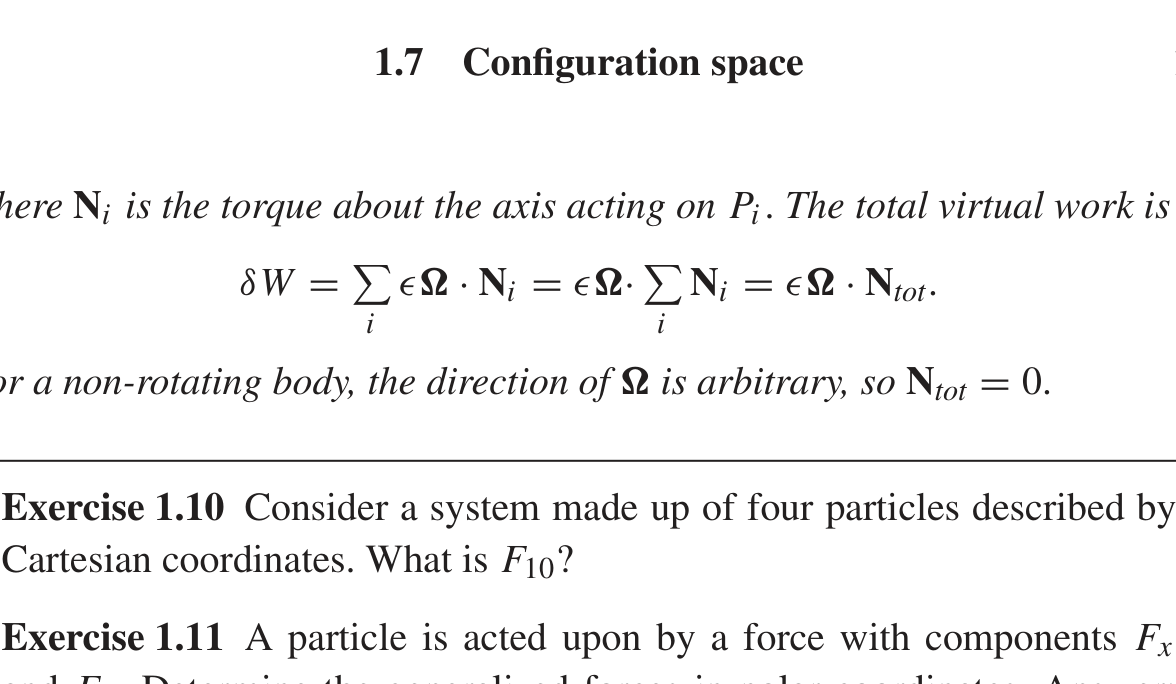
\includegraphics[width=0.55\linewidth]{../Figures/fig_1_2.png}
\caption{Figure 1.2}
\end{figure}

equilibrium requires that M = m/ sin \textbackslash{}theta . (This can be done trivially using
elementary methods, but you are asked to solve the problem using virtual
work.)
\section*{1.7  Configuration space}

The specification of the positions of all of the particles in a system is called the
configuration of the system. In general, the configuration of a system consisting of N free particles is given by
(q1, q2, . . . , qn), where n = 3N.
(1.11)
Consider a single particle. Its position in Cartesian coordinates is given by
x, y, z, and in a rectilinear three-dimensional reference frame the position of
the particle is represented by a point. For a system consisting of two particles,
you might represent the configuration of the system by two points. However,
you could (at least conceptually) represent the configuration by a single point
in a six-dimensional reference frame. In this 6-D space there would be six
mutually perpendicular axes labeled, for example, x1, y1, z1, x2, y2, z2.
Similarly, the configuration of a system composed of N particles is represented by a single point in a 3N-dimensional reference frame.
q
Two blocks in equilibrium.

The axes of such a multi-dimensional reference frame are not necessarily
Cartesian. The positions of the various particles could be represented in spherical coordinates, or cylindrical coordinates, or the generalized coordinates,
q1, q2, . . . , qn. Thus, the configuration of a system consisting of two particles
is expressed as (q1, q2, . . . , q6) where q1 = x1, q2 = y1, . . . , q6 = z2 in Cartesian coordinates. In spherical coordinates, q1 = r1, q2 = \textbackslash{}theta 1, . . . , q6 = \textbackslash{}phi 2, and
similarly for any other coordinate system.
Consider the three-dimensional reference frame of a single particle. As time
goes on the values of the coordinates change. This change is continuous and the
point that represents the position of the particle will trace out a smooth curve.
Similarly, in the n-dimensional configuration space with axes representing the
generalized coordinates, the point representing the configuration of the system
will trace out a smooth curve which represents the time development of the
\begin{figure}[h]
\centering
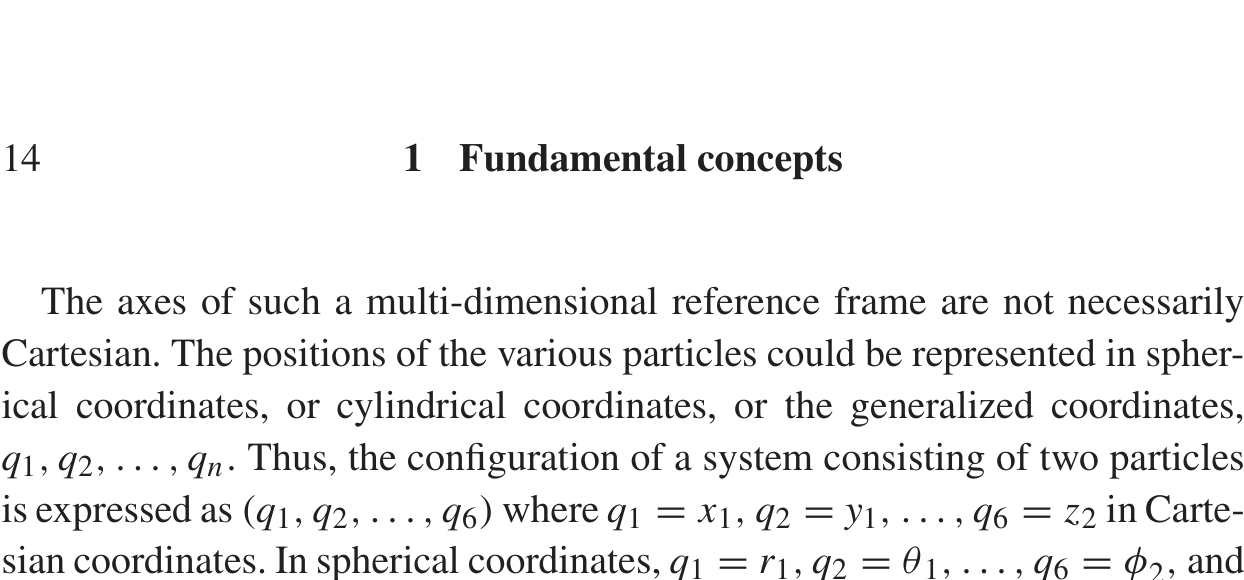
\includegraphics[width=0.55\linewidth]{../Figures/fig_1_3.png}
\caption{Figure 1.3}
\end{figure}

It might be noted that when we transform from one set of coordinates to
a different set of coordinates, the character of the configuration space may
change dramatically. Straight lines may become curves and angles and distances may change. Nevertheless, some geometrical properties remain unaltered. A point is still a point and a curve is still a curve. Adjacent curves
remain adjacent and the neighborhood of a point remains the neighborhood of
the point (although the shape of the neighborhood will probably be different).
\begin{exercise}
Exercise 1.13 A particle moves along a line of constant r from \textbackslash{}theta 1 to \textbackslash{}theta 2.
Show that this is a straight line in r--\textbackslash{}theta  space but not in x--y space.
\end{exercise}

\begin{exercise}
Exercise 1.14 The equation y = 3x + 2 describes a straight line in 2-D
Cartesian space. Determine the shape of this curve in r--\textbackslash{}theta  space.
q1
q2
q3
A path in configuration space. Note that time is a parameter giving
the position of the configuration point along the curve.

1.9
Dynamics
\end{exercise}

\section*{1.8  Phase space}

It is often convenient to describe a system of particles in terms of their positions and their momenta. The ``state'' of a system is described by giving the
values of the positions and momenta of all the particles at some instant of
time. For example we could represent the position of a particle by the Cartesian coordinates $\textbackslash{}xi$, i = 1, 2, 3. Similarly, the momentum of the particle can
be represented by pi, i = 1, 2, 3. Imagine drawing a 2n-dimensional coordinate system in which the axes are labeled thus: x1, . . . , xn; p1, . . . , pn. The
space described by this set of axes is called phase space. The positions of all
the particles as well as the momenta of all the particles are represented by a
single point in phase space. As time progresses the position and the momentum of each particle changes. These change continuously so the point in phase
space moves continuously in the 2n coordinate system. That is, the time development of the system can be represented by a trajectory in phase space. This
trajectory is called the ``phase path'' or, in some contexts, the ``world line.''2
We will shortly define ``generalized momentum'' and then phase space will be
described in terms of the generalized coordinates (q1, . . . , qn) and the generalized momenta (p1, . . . , pn).
\section*{1.9  Dynamics}

1.9.1 Newton's laws of motion
Dynamics is the study of the laws that determine the motion of material bodies. Your first introduction to dynamics was almost certainly a study of Isaac
Newton's three laws.
(1) The first law or the law of inertia: a body not subjected to any external
force will move in a straight line at constant speed.
(2) The second law or the equation of motion: the rate of change of momentum of a body is equal to the net external force applied to it.
(3) The third law or action equals reaction: if a body exerts a force on a
second body, the second body exerts and equal and opposite force of the
same kind on the first one.
The first law tells us that a free particle will move at constant velocity.
2 The concept of phase space is very important in the study of chaotic systems where the
intersection of the trajectory of the system with a particular plane in phase space (the so-called
``surface of section'' ) can be analyzed to determine if chaotic motion is taking place. Also in
statistical mechanics, a basic theorem due to Liouville states that, if one plots the phase space
trajectories of an ensemble of systems, the density of phase space points in the vicinity of a
given system will remain constant in time.

The second law is usually expressed by the vector relation
F = dp
dt .
(1.12)
If the mass is constant this relationship reduces to the well known equation
F = ma.
The third law can be expressed in either in the strong form or in the weak
form. The strong form states that the forces are equal and opposite and directed
along the line joining the particles. The weak form of the third law only states
that the forces are equal and opposite.
These laws (especially the second law) are extremely useful for solving
practical problems.
1.9.2 The equation of motion
The second law is often used to determine the acceleration of a body subjected
to a variety of unbalanced forces. The equation for the acceleration in terms
of positions and velocities is called the ``equation of motion.'' (In introductory
physics courses the determination of the acceleration involved isolating the
system, drawing a free body diagram, and applying the second law, usually
in the form F = ma.) Since forces can be expressed in terms of positions,
velocities and time, the second law yields an expression for the acceleration
having a form such as
$\textbackslash{}ddot x$ = $\textbackslash{}ddot x$(x, $\textbackslash{}dot x$, t).
This is the equation of motion. The position of a particle as a function of time
can then be determined by integrating the equation of motion twice, generating
x = x(t).
The procedure is called determining the motion.
Newton's laws are simple and intuitive and form the basis for most introductory courses in mechanics. It will be convenient to occasionally refer to them,
but our study is not based on Newton's laws.
1.9.3 Newton and Leibniz
It is well known that Isaac Newton and Gottfried Leibniz both invented the
calculus independently. It is less well known that they had different notions
concerning the time development of a system of particles. Newton's second
law gives us a vector relationship between the force on a particle and its

1.9
Dynamics
acceleration. (For a system of N particles, we have N vector relations corresponding to 3N scalar second-order differential equations. These equations are
often coupled in the sense that the positions of all N particles may be present
in each of the 3N equations of motion. To determine the motion we must solve
all these coupled equations simultaneously.)
On the other hand, Leibniz believed that the motions of particles could be
better analyzed by considering their vis-viva or (as we would call it today) their
kinetic energy.
Essentially, Newton considered that the quantity mivi was conserved during the motion, whereas Leibniz believed that miv2
i was constant. In modern terminology, Newton believed in the conservation of momentum whereas
Leibniz believed in the conservation of kinetic energy. It soon became clear
that kinetic energy (T ) is not conserved during the motion of a system, but
when the concept of potential energy (V ) was introduced, Leibniz's theory
was extended to state that the total energy (E = T + V ) is constant, which is,
of course, one of the basic conservation laws of mechanics. Thus, you might
say, both Newton and Leibniz were correct.
In your introductory physics course you often switched between using Newton's laws and using the conservation of energy. For example, the problem of
a falling object can be solved using F = ma or by applying the conservation
of energy.
Later, Euler and Lagrange elaborated on Leibniz's idea and showed that the
motion of a system can be predicted from a single unifying principle, which
we now call Hamilton's principle. Interestingly, this approach does not involve
vectors, or even forces, although forces can be obtained from it. The approach
of Euler and Lagrange is referred to as ``analytical mechanics'' and is the primary focus of our study. (Since Newton's approach is very familiar to you, we
shall occasionally use it when considering some aspect of a physical problem.)
Analytical mechanics does not require Newton's three laws and, in particular,
does away with the third law. Some physicists have suggested that Newton
introduced the third law as a way of dealing with constraints. (A bouncing ball
is ``constrained'' to remain inside the room. In the Newtonian picture, the ball
bounces off a wall because the wall exerts a reaction force on it, as given by the
third law.) The Lagrangian method incorporates constraints into the framework
of the analysis, and neither the second nor the third law is necessary. However,
the forces of constraint as well as the equation of motion can be determined
from the method. Furthermore, all of the equations in analytical mechanics
are scalar equations, so we do not need to use any concepts from vector
analysis. However, sometimes vectors are convenient and we shall use them
occasionally.

This book is concerned with developing the concepts and techniques of analytical mechanics using variational principles.3 I am sure you will find this
to be a very beautiful and very powerful theory. In the introduction to a well
known book on the subject,4 the author, speaking about himself, says, ``Again
and again he experienced the extraordinary elation of mind which accompanies
a preoccupation with the basic principles and methods of analytical mechanics.'' (You may not feel an ``elation of mind'', but I think you will appreciate
what the author was expressing.)
\section*{1.10  Obtaining the equation of motion}

In this section we review the methods for obtaining and solving the equation
of motion. As you might expect, solving the equation of motion yields an
expression for the motion, that is, for the position as a function of time. It happens that there are several different ways of expressing the equation of motion,
but for now let us think of it as an expression for the acceleration of a particle
in terms of the positions and velocities of all the other particles comprising the
system.
As pointed out by Landau and Lifshitz,5 ``If all the coordinates and velocities are simultaneously specified, it is known from experience that the state
of the system is completely determined and that its subsequent motion can, in
principle, be calculated. Mathematically this means that if all the coordinates
q and velocities $\textbackslash{}dot q$ are given at some instant, the accelerations
..q at that instant
are uniquely defined.''
In other words, the equations of motion can be expressed as relations of the
type
..qi =
..qi(q1, q2, . . . , qn;
.q1,
.q2, . . . ,
.qn; t).
If we know the accelerations (
..qi) of the particles, then we can (in principle)
determine the positions and velocities at a subsequent time. Thus, a knowledge of the equations of motion allows us to predict the time development of a
system.
3 Be aware that the fields of analytical mechanics and the calculus of variations are vast and this
book is limited to presenting some fundamental concepts.
4 Cornelius Lanczos, The Variational Principles of Mechanics, The University of Toronto Press,
1970. Reprinted by Dover Press, New York, 1986.
5 L. D. Landau and E. M. Lifshitz, Mechanics, Vol 1 of A Course of Theoretical Physics,
Pergamon Press, Oxford, 1976, p.1.

1.10
Obtaining the equation of motion
1.10.1 The equation of motion in Newtonian mechanics
If the masses are constant, an elementary way to obtain the equation of motion
is to use Newton's second law in the form
$\textbackslash{}ddot r$ = F/m.
(1.13)
This is a second-order differential equation for r that can, in principle, be
solved to yield r = r(t). Of course, this requires having an expression for the
force as a function of r, $\textbackslash{}dot r$, and t.
As a simple one-dimensional example, consider a mass m connected to a
spring of constant k. The force exerted by the spring on the mass is F = -kx.
Therefore, Newton's second law yields the following equation of motion
m$\textbackslash{}ddot x$ + kx = 0.
(1.14)
It is important to note that the second law is applicable only in inertial coordinate systems. Newton was aware of this problem and he stated that the second law is a relationship that holds in a coordinate system at rest with respect
to the fixed stars.
1.10.2 The equation of motion in Lagrangian mechanics
Another way to obtain the equation of motion is to use the Lagrangian technique.
When dealing with particles or with rigid bodies that can be treated as particles, the Lagrangian can be defined to be the difference between the kinetic
energy and the potential energy.6 That is,
L = T -V.
(1.15)
For example, if a mass m is connected to a spring of constant k, the potential
energy is V = 1
2kx2 and the kinetic energy is T = 1
2mv2 = 1
2m$\textbackslash{}dot x$2. Therefore
the Lagrangian is
L = T -V = 1
2m$\textbackslash{}dot x$2 -1
2kx2.
It is usually easy to express the potential energy in whatever set of coordinates being used, but the expression for the kinetic energy may be somewhat
difficult to determine, so whenever possible, one should start with Cartesian
6 Although Equation (1.15) is pefectly correct for a system of particles, we shall obtain a
somewhat different expression when considering continuous systems in Chapter 7. In general,
the Lagrangian is defined to be a function that generates the equations of motion.

coordinates. In the Cartesian coordinate system the kinetic energy takes on the
particularly simple form of a sum of the velocities squared. That is,
T = 1
2m($\textbackslash{}dot x$2 + $\textbackslash{}dot y$2 + $\textbackslash{}dot z$2).
To express the kinetic energy in terms of some other coordinate system requires
a set of transformation equations.
For example, for a pendulum of length l, the potential energy is V
=
-mgl cos \textbackslash{}theta  and the kinetic energy is T = 1
2mv2 = 1
2m(l $\textbackslash{}dot\textbackslash{}$theta )2. (Here \textbackslash{}theta  is the
angle between the string and the perpendicular.) Therefore the Lagrangian is
L = T -V = 1
2ml2 $\textbackslash{}dot\textbackslash{}$theta 2 + mgl cos \textbackslash{}theta .
The kinetic energy is a function of the velocity. (You are familiar with
expressions such as T = 1
2m$\textbackslash{}dot x$2 and T = 1
2ml2 $\textbackslash{}dot\textbackslash{}$theta 2.) The velocity is the time
derivative of a position coordinate ($\textbackslash{}dot x$ and l $\textbackslash{}dot\textbackslash{}$theta ). The potential energy is usually a function only of the position. In generalized coordinates, the position is
expressed as q and the velocity as $\textbackslash{}dot q$. The Lagrangian is, therefore, a function
of q and $\textbackslash{}dot q$. That is, L = L(q, $\textbackslash{}dot q$), or more generally, L = L(q, $\textbackslash{}dot q$, t). If we
are concerned with a single particle free to move in three dimensions, there are
three qs and three $\textbackslash{}dot q$s. Then L = L(q1, q2, q3, $\textbackslash{}dot q$1, $\textbackslash{}dot q$2, $\textbackslash{}dot q$3, t). For a system of N
particles, if n = 3N we write
L = L(qi, $\textbackslash{}dot q$i, t);
i = 1, . . . , n.
I assume you were introduced to the Lagrangian and Lagrange's equations
in your course on intermediate mechanics. In the next two chapters you will
find derivations of Lagrange's equations from first principles. However, for the
moment, I will simply express the equation without proof and show you how
to use it as a tool for obtaining the equation of motion.
For a single coordinate q, Lagrange's equation is
dt
\textbackslash{}partial L
\textbackslash{}partial $\textbackslash{}dot q$ -\textbackslash{}partial L
\textbackslash{}partial q = 0.
(1.16)
If there are n coordinates, there are n Lagrange equations, namely,
dt
\textbackslash{}partial L
\textbackslash{}partial $\textbackslash{}dot q$i
-\textbackslash{}partial L
\textbackslash{}partial qi
= 0, i = 1, . . . , n.
(1.17)
It is important to realize that Lagrange's equations are the equations of
motion of a system.

1.10
Obtaining the equation of motion
For example, for a mass on a spring the Lagrangian is L = T -V =
2m$\textbackslash{}dot x$2 -1
2kx2. Plugging this into the Lagrange equation we obtain
dt
\textbackslash{}partial L
\textbackslash{}partial $\textbackslash{}dot x$

-\textbackslash{}partial L
\textbackslash{}partial x = 0,
dt
\textbackslash{}partial
\textbackslash{}partial $\textbackslash{}dot x$
2m$\textbackslash{}dot x$2 -1
2kx2

-\textbackslash{}partial
\textbackslash{}partial x
2m$\textbackslash{}dot x$2 -1
2kx2

= 0,
dt (m$\textbackslash{}dot x$) -kx = 0,
so
m$\textbackslash{}ddot x$ + kx = 0,
as expected. (Compare with Equation 1.14.)
To illustrate the use of Lagrange's equations to obtain the equations of
motion, we consider several simple mechanical systems.
\begin{figure}[h]
\centering
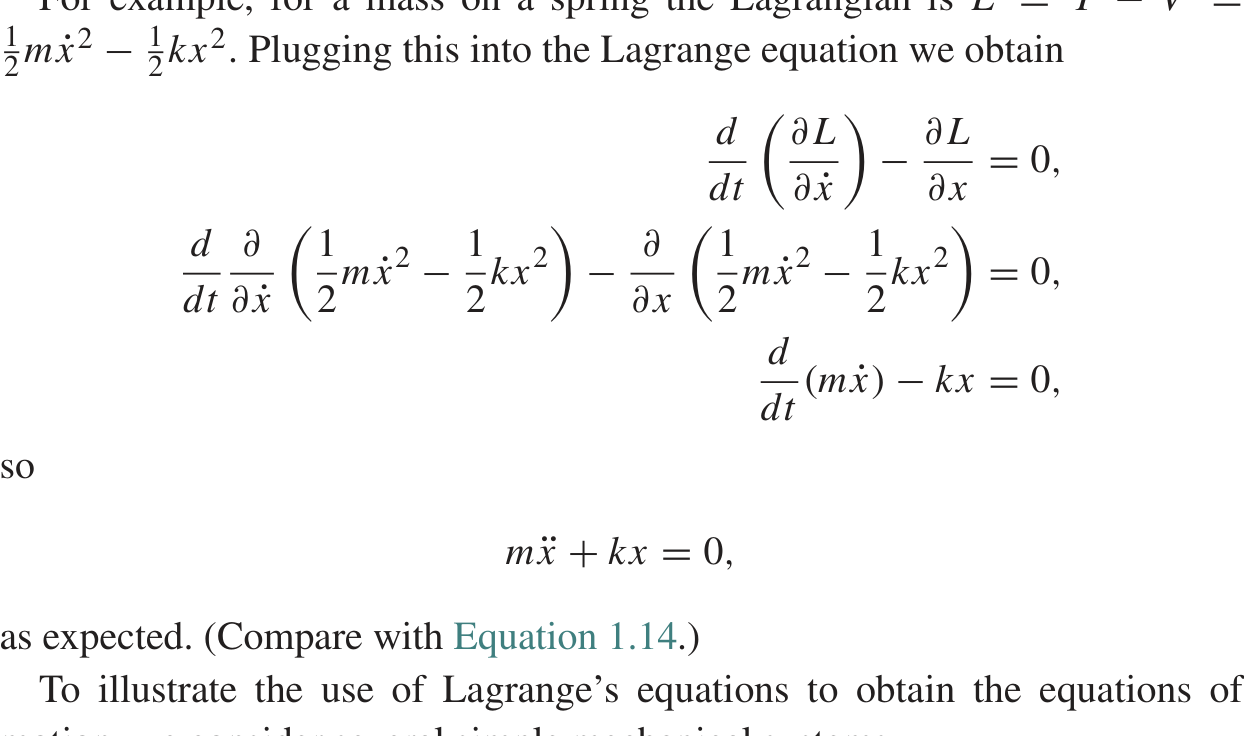
\includegraphics[width=0.55\linewidth]{../Figures/fig_1_4.png}
\caption{Figure 1.4}
\end{figure}

It consists of masses m1 and m2 suspended by a massless inextensible string
over a frictionless, massless pulley. Evaluate the Lagrangian and obtain the
equation of motion.
Solution 1.2 The kinetic energy of the masses is
T = 1
2m1 $\textbackslash{}dot x$2
1 + 1
2m2 $\textbackslash{}dot x$2
2,
and the potential energy is
V = -m1gx1 -m2gx2,
where we selected V = 0 at the center of the pulley. The system is subjected to
the constraint x1 + x2 = l = constant. The Lagrangian is,
V = 0
m2
m1
x1
x2 = l - x1
Atwood's machine.

L = T -V = 1
2m1 $\textbackslash{}dot x$2
1 + 1
2m2 $\textbackslash{}dot x$2
2 + m1gx1 + m2gx2.
But using x2 = l -x1 we can rewrite the Lagrangian in terms of a single
variable,
L = 1
2m1 $\textbackslash{}dot x$2
1 + 1
2m2 $\textbackslash{}dot x$2
1 + m1gx1 + m2g(l -x1),
= 1
2(m1 + m2)$\textbackslash{}dot x$2
1 + (m1 -m2)gx1 + m2gl.
The equation of motion is
dt
\textbackslash{}partial L
\textbackslash{}partial $\textbackslash{}dot x$1
-\textbackslash{}partial L
\textbackslash{}partial x1
= 0,
dt (m1 + m2)$\textbackslash{}dot x$1 -(m1 -m2)g = 0,
$\textbackslash{}ddot x$1 = m1 -m2
m1 + m2
g.
\begin{example}
Example 1.3 A cylinder of radius a and mass m rolls without slipping on a
fixed cylinder of radius b. Evaluate the Lagrangian and obtain the equation of
\begin{figure}[h]
\centering
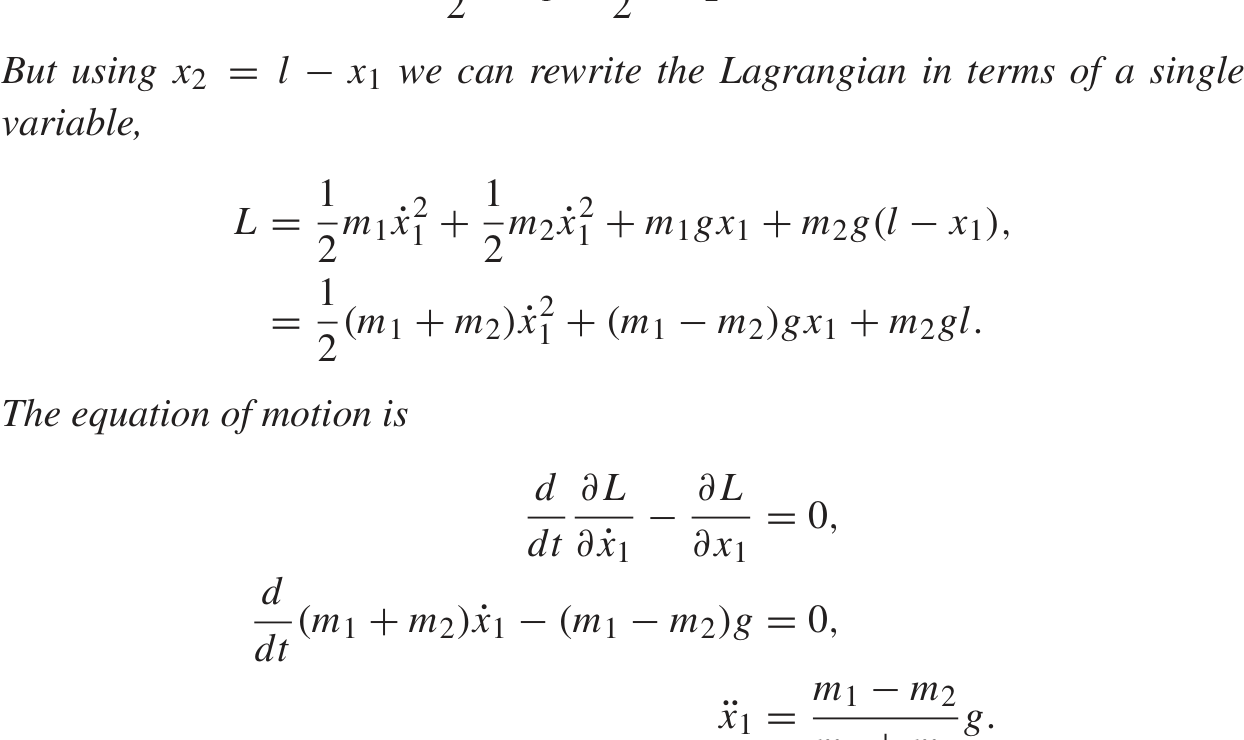
\includegraphics[width=0.55\linewidth]{../Figures/fig_1_5.png}
\caption{Figure 1.5}
\end{figure}

Solution 1.3 The kinetic energy of the smaller cylinder is the kinetic energy
of translation of its center of mass plus the kinetic energy of rotation about its
center of mass. That is,
T = 1
2m

$\textbackslash{}dot r$2 + r2 $\textbackslash{}dot\textbackslash{}$theta 2
+ 1
2I $\textbackslash{}dot\textbackslash{}$phi 2,
where r is the distance between the centers of the cylinders and I = 1
2ma2.
The potential energy is V = mgr cos \textbackslash{}theta . Therefore
q
b
a
f
V = 0
A cylinder rolling on another cylinder.

1.10
Obtaining the equation of motion
L = 1
2m($\textbackslash{}dot r$2 + r2 $\textbackslash{}dot\textbackslash{}$theta 2) + 1
2I $\textbackslash{}dot\textbackslash{}$phi 2 -mgr cos \textbackslash{}theta .
But there are two constraints, namely, r = a + b and a\textbackslash{}phi  = b\textbackslash{}theta . Therefore
$\textbackslash{}dot r$ = 0 and $\textbackslash{}dot\textbackslash{}$phi  = (b/a)$\textbackslash{}dot\textbackslash{}$theta . So,
L = 1
2m(a + b)2 $\textbackslash{}dot\textbackslash{}$theta 2 + 1
2ma2
b
a
$\textbackslash{}dot\textbackslash{}$theta
-mg(a + b) cos \textbackslash{}theta
= 1
2m

a2 + 2ab + 3
2b2

$\textbackslash{}dot\textbackslash{}$theta 2 -mg(a + b) cos \textbackslash{}theta
and the equation of motion is
dt
\textbackslash{}partial L
\textbackslash{}partial $\textbackslash{}dot q$ -\textbackslash{}partial L
\textbackslash{}partial q = 0
or

a2 + 2ab + 3
2b2

$\textbackslash{}ddot \textbackslash{}theta$  -mg(a + b) sin \textbackslash{}theta  = 0.
\end{example}

\begin{example}
Example 1.4 A bead of mass m slides on a massive frictionless hoop of radius
a. The hoop is rotating at a constant angular speed \textbackslash{}omega  about a vertical axis. See
\begin{figure}[h]
\centering
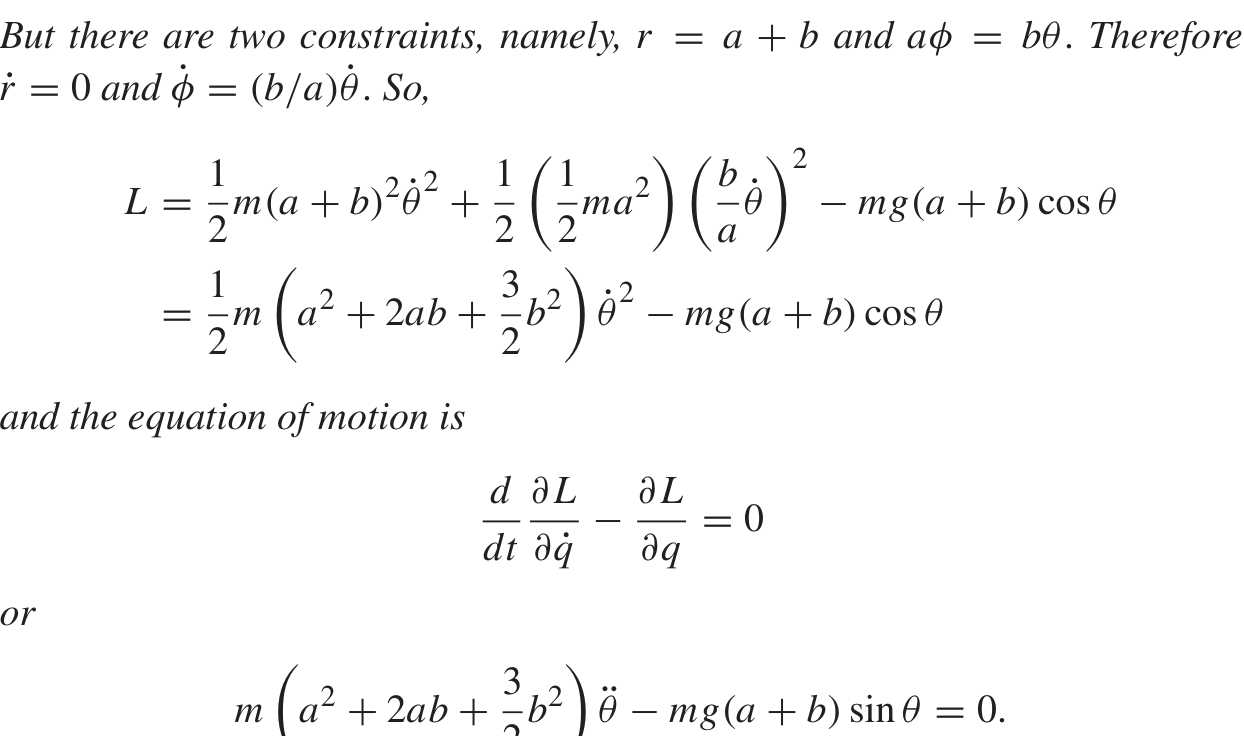
\includegraphics[width=0.55\linewidth]{../Figures/fig_1_6.png}
\caption{Figure 1.6}
\end{figure}

Solution 1.4 If the hoop is massive enough, the motion of the bead will not
affect the rotation rate of the hoop. Thus we ignore the energy of the hoop. The
kinetic energy is the energy of the bead due to the rotation of the hoop as well
as kinetic energy of the bead due to its motion on the hoop which is associated
with changes in the angle \textbackslash{}theta . Therefore,
L = 1
2ma2 $\textbackslash{}dot\textbackslash{}$theta 2 + 1
2ma2\textbackslash{}omega 2 sin2 \textbackslash{}theta  + mga cos \textbackslash{}theta .
w
a
q
mg
A bead slides on a rotating hoop.

V = 0
f
q
y
z
A spherical pendulum.
The equation of motion is
ma2$\textbackslash{}ddot \textbackslash{}theta$  -ma2\textbackslash{}omega 2 sin \textbackslash{}theta  cos \textbackslash{}theta  + mga sin \textbackslash{}theta  = 0.
\end{example}

\begin{example}
Example 1.5 A spherical pendulum consists of a bob of mass m suspended
from an inextensible string of length l. Determine the Lagrangian and the
\begin{figure}[h]
\centering
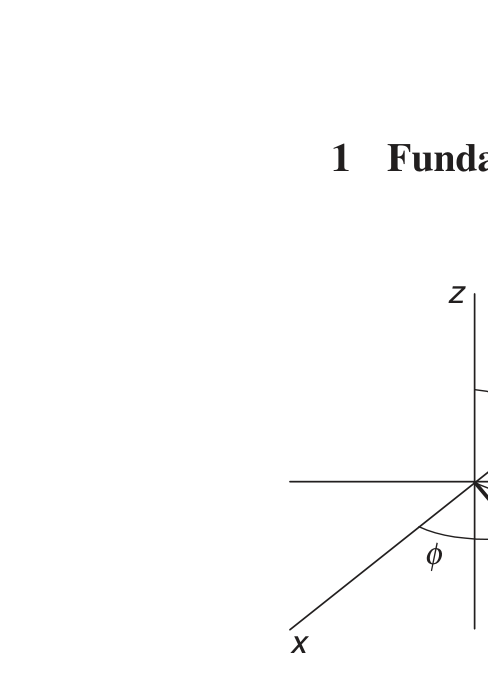
\includegraphics[width=0.55\linewidth]{../Figures/fig_1_7.png}
\caption{Figure 1.7}
\end{figure}

from the positive z axis, and \textbackslash{}phi , the azimuthal angle, is measured from the x
axis in the x--y plane.
Solution 1.5 The Lagrangian is
L = 1
2m($\textbackslash{}dot x$2 + $\textbackslash{}dot y$2 + $\textbackslash{}dot z$2) -mgz.
But
x = l sin \textbackslash{}theta  cos \textbackslash{}phi
y = l sin \textbackslash{}theta  sin \textbackslash{}phi
z = l cos \textbackslash{}theta
so
L = 1
2ml2($\textbackslash{}dot\textbackslash{}$theta 2 + sin2 \textbackslash{}theta  $\textbackslash{}dot\textbackslash{}$phi 2) -mgl cos \textbackslash{}theta .
The equations of motion are
dt

ml2 $\textbackslash{}dot\textbackslash{}$theta

-ml2 $\textbackslash{}dot\textbackslash{}$phi 2 sin \textbackslash{}theta  cos \textbackslash{}theta  -mgl sin \textbackslash{}theta  = 0,
dt (ml2 sin2 \textbackslash{}theta  $\textbackslash{}dot\textbackslash{}$phi ) = 0.

1.11
Conservation laws and symmetry principles
l2
l1
m1
m2
A double planar pendulum.
\end{example}

\begin{exercise}
Exercise 1.15 Obtain the Lagrangian and the equation of motion for an
Atwood's machine if the pulley has a moment of inertia I. Answer: a =
g(m2 -m1)/(m1 + m2 + I/R2).
\end{exercise}

\begin{exercise}
Exercise 1.16 Obtain the Lagrangian for a simple pendulum and for a
\begin{figure}[h]
\centering
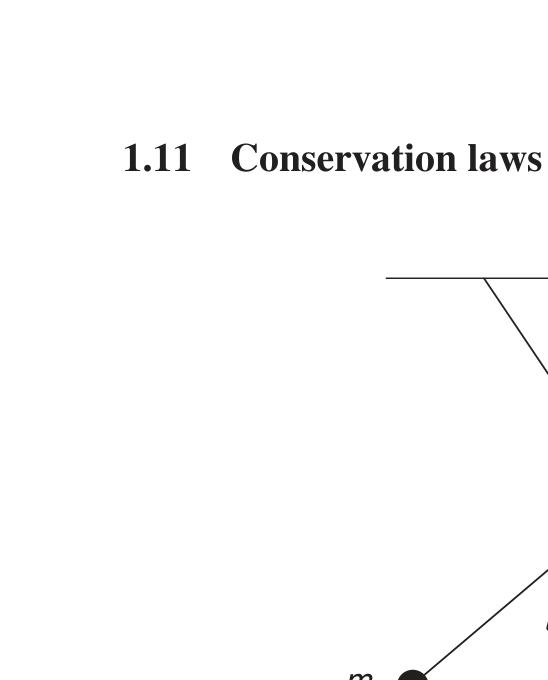
\includegraphics[width=0.55\linewidth]{../Figures/fig_1_8.png}
\caption{Figure 1.8}
\end{figure}

Assume the motion is planar.) Answer: For the double pendulum
L = 1
2(m1 + m2)l2
1 $\textbackslash{}dot\textbackslash{}$theta 2
1 + 1
2m2

l2
2 $\textbackslash{}dot\textbackslash{}$theta 2
2 + 2l1l2 $\textbackslash{}dot\textbackslash{}$theta 1 $\textbackslash{}dot\textbackslash{}$theta 2 cos(\textbackslash{}theta 1 -\textbackslash{}theta 2)

+ m1gl1 cos \textbackslash{}theta 1 + m2g(l1 cos \textbackslash{}theta 1 + l2 cos \textbackslash{}theta 2).
\end{exercise}

\begin{exercise}
Exercise 1.17 A flyball governor is a simple mechanical device to control
the speed of a motor. As the device spins faster and faster, the mass m2
\begin{figure}[h]
\centering
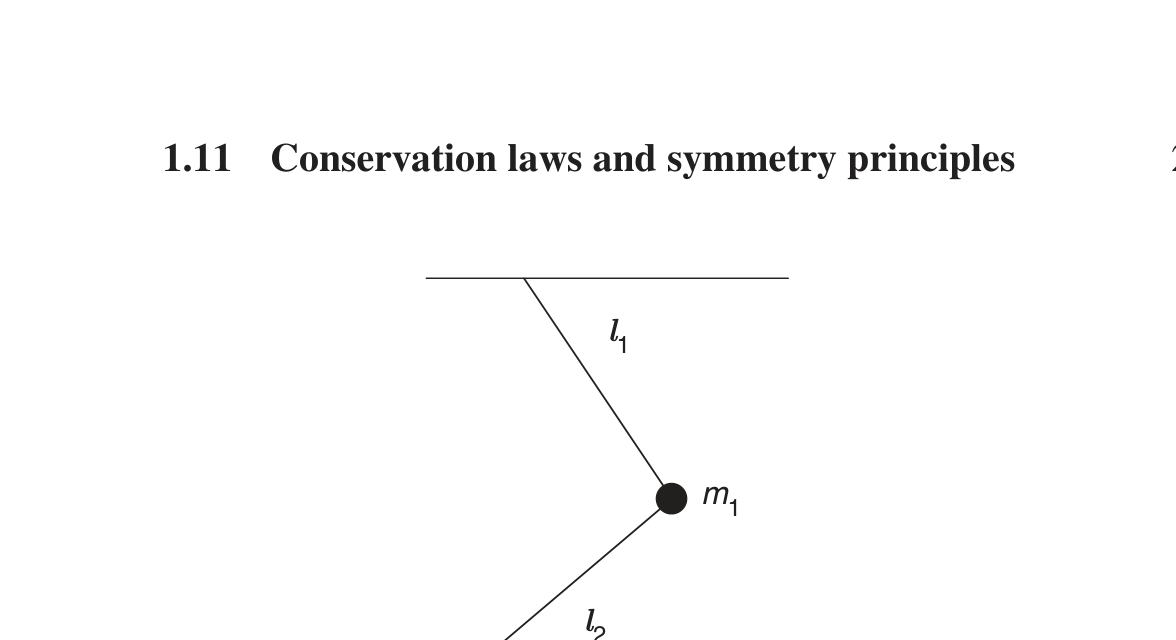
\includegraphics[width=0.55\linewidth]{../Figures/fig_1_9.png}
\caption{Figure 1.9}
\end{figure}

The angle \textbackslash{}theta  is formed by one of the rods and the central axis, and the angle
\textbackslash{}phi  is the rotation angle about the axis. The angular speed at any moment is
\textbackslash{}omega  = $\textbackslash{}dot\textbackslash{}$phi . Assume the system is in a uniform gravitational field. Show that
the Lagrangian is given by
L = m1a2
$\textbackslash{}dot\textbackslash{}$theta 2 + \textbackslash{}omega 2 sin2 \textbackslash{}theta

+ 2m2a2 $\textbackslash{}dot\textbackslash{}$theta 2 sin2 \textbackslash{}theta  + 2 (m1 + m2) ga cos \textbackslash{}theta .
\end{exercise}

\section*{1.11  Conservation laws and symmetry principles}

The three most important conservation laws in classical mechanics are the conservation of linear momentum, the conservation of angular momentum and
the conservation of energy. Although you are very familiar with these laws,

w
V = 0
q
a
a
a
a
m1
m1
m2
A flyball governor.
it is interesting to consider them in terms of generalized coordinates and the
Lagrangian. We will show that these three basic conservation laws are consequences of the homogeneity and isotropy of space and the homogeneity
of time.
When we say a region of space is homogeneous we mean that it is the same
in one location as in another. Consequently, a system will be unaffected by a
displacement from one point to another. As a simple example, I claim that my
grandfather clock behaved the same on one side of the room as on the other
(but it would behave differently on the Moon).
Similarly, if space is isotropic, it looks the same in all directions and a physical system is unchanged under a rotation. My grandfather clock behaved the
same after I rotated it through 90◦about a vertical axis. However, the space in
my room is not isotropic for a rotation about a horizontal axis. (When I turned
my grandfather clock upside-down it stopped working.)
Finally, if time is homogeneous, a physical system will behave the same at
two different times. My clock behaved the same today as it did last week.
Time is also isotropic in the sense that physical systems behave the same
whether time is running forward or backward.
When we say that a system has a particular symmetry, we mean that the
system is invariant with respect to a change in some particular coordinate.
For example, a sphere is an object that appears the same no matter how it
is rotated. Spherical symmetry implies an invariance with respect to rotations,
i.e., with respect to a change in the angular orientation of the object. Similarly,
if a system is unchanged when it undergoes a displacement in some particular

1.11
Conservation laws and symmetry principles
direction, we say that it has translational symmetry in that direction. When a
system is invariant with respect to a change in time, we say it has temporal
symmetry.
As an example of translational symmetry consider an object sitting on an
infinite horizontal surface in a uniform, vertical gravitational field. If the object
is moved in the horizontal plane, the system is unchanged. If, however, the
object is moved vertically (if it is raised), the potential energy changes. Thus
this system has translational symmetry in the horizontal plane but it does not
have translational symmetry for vertical displacements. In a region where no
forces are acting, space is homogeneous in all three directions.
A mechanical system is completely described by its Lagrangian. If the
Lagrangian does not depend explicitly on some particular coordinate qi, then
a change in qi does not affect the system. The system is said to be symmetric
with respect to changes in qi.
1.11.1 Generalized momentum and cyclic coordinates
Generalized momentum
A free particle is described by the Lagrangian
L = 1
2m($\textbackslash{}dot x$2 + $\textbackslash{}dot y$2 + $\textbackslash{}dot z$2).
Taking the partial derivative with respect to $\textbackslash{}dot x$ we obtain
\textbackslash{}partial L
\textbackslash{}partial $\textbackslash{}dot x$ = m$\textbackslash{}dot x$.
But m$\textbackslash{}dot x$ is just the x component of the linear momentum. That is,
px = \textbackslash{}partial L
\textbackslash{}partial $\textbackslash{}dot x$ .
(1.18)
Similarly,
py = \textbackslash{}partial L
\textbackslash{}partial $\textbackslash{}dot y$
pz = \textbackslash{}partial L
\textbackslash{}partial $\textbackslash{}dot z$ .
The Lagrangian for a freely rotating wheel with moment of inertia I is
L = 1
2I $\textbackslash{}dot\textbackslash{}$theta 2
and
\textbackslash{}partial L
\textbackslash{}partial $\textbackslash{}dot\textbackslash{}$theta  = I $\textbackslash{}dot\textbackslash{}$theta .
But I $\textbackslash{}dot\textbackslash{}$theta  is the angular momentum.

In both of these examples, the momentum was the derivative of the
Lagrangian with respect to a velocity. We carry this idea to its logical conclusion and define the generalized momentum by
pi = \textbackslash{}partial L
\textbackslash{}partial $\textbackslash{}dot q$i
.
The generalized momentum pi is associated with the generalized coordinate
qi and is sometimes referred to as the conjugate momentum. Thus, we have
seen that the linear momentum px is conjugate to the linear coordinate x and
the angular momentum I $\textbackslash{}dot\textbackslash{}$theta  is conjugate to the angular coordinate \textbackslash{}theta .
Cyclic coordinates
If a particular coordinate does not appear in the Lagrangian, it is called ``cyclic''
or ``ignorable.'' For example, the Lagrangian for a mass point in a gravitational
field is
L = 1
2m($\textbackslash{}dot x$2 + $\textbackslash{}dot y$2 + $\textbackslash{}dot z$2) -mgz.
Since neither x nor y appear in the Lagrangian, they are cyclic. (Note, however, that the time derivatives of the coordinates, $\textbackslash{}dot x$ and $\textbackslash{}dot y$, do appear in the
Lagrangian, so there is an implicit dependence on x and y.)
Lagrange's equation tells us that
dt
\textbackslash{}partial L
\textbackslash{}partial $\textbackslash{}dot q$i
-\textbackslash{}partial L
\textbackslash{}partial qi
= 0.
But if qi is cyclic, the second term is zero and
dt
\textbackslash{}partial L
\textbackslash{}partial $\textbackslash{}dot q$i
= 0.
Since
pi = \textbackslash{}partial L
\textbackslash{}partial $\textbackslash{}dot q$i
we have
dt pi = 0
or
pi = constant.
That is, the generalized momentum conjugate to a cyclic coordinate is a
constant.

1.11
Conservation laws and symmetry principles
\begin{exercise}
Exercise 1.18 Identify any conserved momenta for the spherical pendulum.
\end{exercise}

\begin{exercise}
Exercise 1.19 Write the Lagrangian for a planet orbiting the Sun.
Determine any cyclic coordinates and identify the conserved conjugate
momenta. Answer: L = (1/2)(m$\textbackslash{}dot r$2 + mr2 $\textbackslash{}dot\textbackslash{}$theta 2) + GmM/r2.
\end{exercise}

\begin{exercise}
Exercise 1.20 Show that as long as the kinetic energy depends only on
velocities and not on coordinates, then the generalized force is given by
Qi = \textbackslash{}partial L
\textbackslash{}partial qi .
The relation between symmetries and conserved quantities
We have determined that the generalized momentum conjugate to an ignorable (cyclic) coordinate is conserved. If the coordinate qi is cyclic, it does not
appear in the Lagrangian and the system does not depend on the value of qi.
Changing qi has no effect on the system; it is the same after qi is changed as it
was before. If qi = \textbackslash{}theta , then a rotation through \textbackslash{}theta  changes nothing. But that is,
essentially, the definition of symmetry. Consequently, if a coordinate is cyclic,
the system is symmetric under changes in that coordinate. Furthermore, each
symmetry in a coordinate gives rise to a conserved conjugate momentum. For
example, for an object sitting on a horizontal surface, the horizontal components of linear momentum are constant. If the x and y axes are in the horizontal
plane, then there is no force in either the x or y directions. If there were a force
in, say, the x direction, then the potential energy would depend on x and consequently the Lagrangian would contain x and it would not be an ignorable
coordinate.
The idea that conserved quantities are related to symmetries is highly
exploited in studies of the elementary particles. For example, particle physicists frequently utilize the law of conservation of parity and the law of conservation of ``strangeness.'' These conservation laws are associated with observed
symmetries in the behavior of elementary particles. Parity conservation is an
expression of the symmetry of right-handedness and left-handedness in reactions involving elementary particles. (As you probably know, there are some
reactions in which parity is not conserved.)
As an example from the field of elementary particle physics, it is observed
that some reactions never occur. There is no apparent reason why a reaction
such as \textbackslash{}pi -+ p \textbackslash{}to \textbackslash{}pi o +  does not take place. It must violate some conservation law. However, it does not violate any of the everyday conservation
laws such as charge, mass-energy, parity, etc. But since the reaction does not

occur, using the principle that ``what is not forbidden is required,'' physicists
concluded that there must be a conservation principle at work. They called it
conservation of strangeness. Studying reactions that do occur allowed them
to assign to each particle a ``strangeness quantum number.'' For example, the
strangeness of a \textbackslash{}pi  particle is 0, that of a proton is also 0 and the strangeness
of a  particle is -1. The total strangeness on the right-hand side of the reaction is not equal to the total strangeness on the left-hand side. Therefore, in this
reaction, strangeness is not conserved and the reaction does not take place. This
is not any weirder than requiring that linear momentum be conserved during
a collision. However, we feel at home with momentum conservation because
we have an analytical expression for momentum and we known that conservation of momentum implies that no net external forces are acting on the system.
We do not have an analytical expression for strangeness nor do we know what
symmetry is implied by strangeness conservation. We have no idea what the
associated cyclic coordinate might be. None the less, the basic idea is the same.
In conclusion, we can state that for every symmetry, there is a corresponding
constant of the motion. This is, essentially, Noether's theorem.7
\end{exercise}

\begin{exercise}
Exercise 1.21 Find the ignorable coordinates for the spherical pendulum
and determine the associated symmetry.
1.11.2 The conservation of linear momentum
In this section we will study the theoretical basis for the law of conservation of
linear momentum. However, before we begin, let us note that there are several
different ways to arrive at this conservation law.
For example, in your introductory physics course, you learned the law of
conservation of linear momentum by considering Newton's second law in the
form
F = dP
dt .
If there is no net external force acting on the system, F = 0, and hence the time
derivative of the total momentum P is zero, that is, the total linear momentum
of the system is constant.
In your intermediate mechanics course, you probably considered the conservation of linear momentum from a more sophisticated point of view. Perhaps
7 Emmy Noether (1882--1932), a mathematical physicist, proved the theorem that is named
after her.

1.11
Conservation laws and symmetry principles
you considered a situation in which the potential energy did not depend on
some particular coordinate, say x, and the kinetic energy also did not contain
x. When you wrote the Lagrangian, L = T -V, you obtained an expression
that did not contain x and consequently x was a cyclic coordinate. That is,
\textbackslash{}partial L
\textbackslash{}partial x = 0.
Now the Lagrange equation for x is
dt
\textbackslash{}partial L
\textbackslash{}partial $\textbackslash{}dot x$ -\textbackslash{}partial L
\textbackslash{}partial x = 0,
which reduces to
dt
\textbackslash{}partial L
\textbackslash{}partial $\textbackslash{}dot x$ = 0.
But \textbackslash{}partial L
\textbackslash{}partial $\textbackslash{}dot x$ = px, so
dt px = 0.
Again we see that if the Lagrangian does not depend on x, then px is
constant.
We now show that the conservation of linear momentum is a consequence of
the homogeneity of space, that is, we shall show that in a region of space whose
properties are the same everywhere, the total linear momentum of a mechanical
system will be constant. Our argument not only guarantees the conservation of
linear momentum, but also leads to Newton's second and third laws, as we now
demonstrate.
Consider a system composed of N particles situated at r\textbackslash{}alpha  (\textbackslash{}alpha  = 1, . . . , N).
(For the sake of variety, the argument here is formulated in terms of vectors.) If
every particle is displaced by the same infinitesimal distance ϵ, the positions of
all particles will change according to r\textbackslash{}alpha  \textbackslash{}to r\textbackslash{}alpha  + ϵ. We assume that ϵ is a virtual displacement in which the all the particles are displaced infinitesimally but
the velocities are unchanged and time is frozen. Recall that if f = f (qi, $\textbackslash{}dot q$i, t),
then the differential of f, according to the rules of calculus, is
df =
n
i=1
\textbackslash{}partial f
\textbackslash{}partial qi
dqi +
n
i=1
\textbackslash{}partial f
\textbackslash{}partial $\textbackslash{}dot q$i
d $\textbackslash{}dot q$i + \textbackslash{}partial f
\textbackslash{}partial t dt.
But the change in f due to an infinitesimal virtual displacement is
\textbackslash{}delta f = \textbackslash{}partial f
\textbackslash{}partial q1
\textbackslash{}delta q1 + \textbackslash{}partial f
\textbackslash{}partial q2
\textbackslash{}delta q2 + \textbackslash{}cdot  \textbackslash{}cdot  \textbackslash{}cdot
=
N
\textbackslash{}alpha =1
\textbackslash{}partial f
\textbackslash{}partial ra
\textbackslash{}cdot  \textbackslash{}delta r\textbackslash{}alpha ,

where we have used the fact that time is frozen and that a displacement of the
entire system will have no effect on velocities.8
Consequently, the change in a Lagrangian due to a virtual displacement ϵ is
\textbackslash{}delta L =
\textbackslash{}alpha
\textbackslash{}partial L
\textbackslash{}partial r\textbackslash{}alpha
\textbackslash{}cdot  \textbackslash{}delta r\textbackslash{}alpha  =
\textbackslash{}alpha
\textbackslash{}partial L
\textbackslash{}partial r\textbackslash{}alpha
\textbackslash{}cdot  ϵ = ϵ\textbackslash{}cdot
\textbackslash{}alpha
\textbackslash{}partial L
\textbackslash{}partial r\textbackslash{}alpha
,
where we used that fact that \textbackslash{}delta r\textbackslash{}alpha  = ϵ, that is, all particles are displaced the
same amount. Note that we are summing over particles (\textbackslash{}alpha  = 1, . . . , N), not
components (i = 1, . . . , 3N).
If the space is homogeneous, the Lagrangian does not change and \textbackslash{}delta L = 0.
Therefore,

\textbackslash{}alpha
\textbackslash{}partial L
\textbackslash{}partial r\textbackslash{}alpha
= 0.
But by Lagrange's equations,
\textbackslash{}partial L
\textbackslash{}partial r\textbackslash{}alpha
= d
dt
\textbackslash{}partial L
\textbackslash{}partial v\textbackslash{}alpha
,
so
dt

\textbackslash{}alpha
\textbackslash{}partial L
\textbackslash{}partial v\textbackslash{}alpha
= d
dt

\textbackslash{}alpha
p\textbackslash{}alpha  = d
dt Ptot = 0.
This means that
Ptot = constant,
as expected.
We are not using any particular set of coordinates, as we have been formulating the problem in terms of vectors. The vector definition of kinetic energy
is T = (1/2)mv \textbackslash{}cdot  v. As long as we express our relations in terms of vectors
8 We are using the notation of Landau and Lifshitz involving the derivative of a scalar with
respect to a vector. For example, if there is only one particle (\textbackslash{}alpha  = 1), we define
\textbackslash{}partial F
\textbackslash{}partial r \textbackslash{}equiv \textbackslash{}hat\{i\} \textbackslash{}partial F
\textbackslash{}partial x + \textbackslash{}hat\{j\} \textbackslash{}partial F
\textbackslash{}partial y + \textbackslash{}hat\{k\} \textbackslash{}partial F
\textbackslash{}partial z .
Thus, the derivative of a scalar with respect to a vector is defined as the vector whose
components are the derivatives of the scalar with respect to the components of the vector.
Note that
\textbackslash{}partial F
\textbackslash{}partial r = \textbackslash{}nabla F.

1.11
Conservation laws and symmetry principles
the kinetic energy depends only on the square of the velocity and not on the
coordinates9 and we can write
\textbackslash{}partial L
\textbackslash{}partial r\textbackslash{}alpha
= -\textbackslash{}partial V
\textbackslash{}partial r\textbackslash{}alpha
= F\textbackslash{}alpha .
But if

\textbackslash{}alpha
\textbackslash{}partial L
\textbackslash{}partial r\textbackslash{}alpha
= 0,
then

\textbackslash{}alpha
F\textbackslash{}alpha  = 0.
That is, the sum of all the forces acting on all the particles in the system is
zero. If the system consists of just two particles, this tells us that F1 + F2 = 0,
which is Newton's third law. Additionally,
\textbackslash{}partial L
\textbackslash{}partial r\textbackslash{}alpha
= d
dt
\textbackslash{}partial L
\textbackslash{}partial v\textbackslash{}alpha
= d
dt p\textbackslash{}alpha  = F\textbackslash{}alpha ,
and we have also obtained Newton's second law.
1.11.3 The conservation of angular momentum
Our next task is to show that the conservation of angular momentum is a consequence of the isotropy of space. But before we tackle that problem, let us
consider the conservation law first from an elementary and then from an intermediate point of view.
The elementary level consideration of the law of conservation of angular
momentum usually starts with the definition of the angular momentum of a
particle:
l = r \textbackslash{}times  p,
where r is the position of the particle and p =mv is its linear momentum.
Differentiating with respect to time yields
dt = d
dt (r \textbackslash{}times  p) = dr
dt \textbackslash{}times  p + r\textbackslash{}times dp
dt .
9 This is also true in Cartesian coordinates in which T = (1/2)m

$\textbackslash{}dot x$2 + $\textbackslash{}dot y$2 + $\textbackslash{}dot z$2
. But in most
other coordinate systems the kinetic energy will depend on coordinates as well as velocities.
For example, in spherical coordinates
T = (1/2)m($\textbackslash{}dot r$2 + r2 $\textbackslash{}dot\textbackslash{}$theta 2 + r2 sin2 \textbackslash{}theta  $\textbackslash{}dot\textbackslash{}$phi 2).

Since dr
dt = v, the first term is m(v \textbackslash{}times  v) = 0. The second term contains dp
dt
which, by Newton's second law, is the net force acting on the particle. Therefore the second term is r \textbackslash{}times  F = N = torque. That is
dt = N.
One can then show that the law holds for a system of particles (which requires
invoking Newton's third law), and one concludes that the angular momentum
of a system of particles is constant if there is no net external external torque
acting on it.
A familiar example is the constancy of angular momentum of a particle in
a central force field (such as a planet under the influence of the Sun). Since a
central force has the form F = f (r)\textbackslash{}hat\{r\}, the torque acting on the particle is
N = r \textbackslash{}times  F =rf (r)(\textbackslash{}hat\{r\} \textbackslash{}times  \textbackslash{}hat\{r\}) = 0,
and the conjecture is proved.
An intermediate level discussion of the conservation of angular momentum
might begin by considering a particle moving in a plane in a region of space
where the potential energy is V = V (r). (For example, V = -GMm/r.) The
transformation equations from Cartesian to polar coordinates are
x = r cos \textbackslash{}theta
y = r sin \textbackslash{}theta .
Therefore,
$\textbackslash{}dot x$ = $\textbackslash{}dot r$ cos \textbackslash{}theta  -r $\textbackslash{}dot\textbackslash{}$theta  sin \textbackslash{}theta
$\textbackslash{}dot y$ = $\textbackslash{}dot r$ sin \textbackslash{}theta  + r $\textbackslash{}dot\textbackslash{}$theta  cos \textbackslash{}theta ,
and
T = 1
2m

$\textbackslash{}dot x$2 + $\textbackslash{}dot y$2
= 1
2m

$\textbackslash{}dot r$2 + r2 $\textbackslash{}dot\textbackslash{}$theta 2
so
L = T -V = 1
2m

$\textbackslash{}dot r$2 + r2 $\textbackslash{}dot\textbackslash{}$theta 2
-V (r).
The momentum conjugate to \textbackslash{}theta  is
p\textbackslash{}theta  = \textbackslash{}partial L
\textbackslash{}partial $\textbackslash{}dot\textbackslash{}$theta  = \textbackslash{}partial
\textbackslash{}partial $\textbackslash{}dot\textbackslash{}$theta
2m

$\textbackslash{}dot r$2 + r2 $\textbackslash{}dot\textbackslash{}$theta 2
-V (r)

= mr2 $\textbackslash{}dot\textbackslash{}$theta ,
which we recognize as the angular momentum of the particle. Observe that \textbackslash{}theta
is ignorable, so the angular momentum, mr2 $\textbackslash{}dot\textbackslash{}$theta  is constant.

1.11
Conservation laws and symmetry principles
q
df
df
ra sin qdf = \textbar{}dra\textbar{}
ra
ra (after rotation)
From above
df
va (after)
va (before)
dra  = df \textbackslash{}times  ra
ra sin q
The rotation of the system changes the position of each particle by
\textbackslash{}delta r\textbackslash{}alpha  and the velocity of each particle by \textbackslash{}delta v\textbackslash{}alpha .
We now address this question in a more advanced manner and show that the
conservation of angular momentum is a consequence of the isotropy of space.
Consider a mechanical system that is rotated through a virtual angle \textbackslash{}delta \textbackslash{}phi  around
some axis. Let \textbackslash{}delta \textbackslash{}phi  be a vector directed along the axis of rotation and having
magnitude \textbackslash{}delta \textbackslash{}phi . Place the origin of coordinates on the axis of rotation. Owing to
the rotation, every particle in the system is displaced by some distance \textbackslash{}delta r\textbackslash{}alpha  and
if a particle has velocity v\textbackslash{}alpha , the direction of the velocity vector will change by
\begin{figure}[h]
\centering
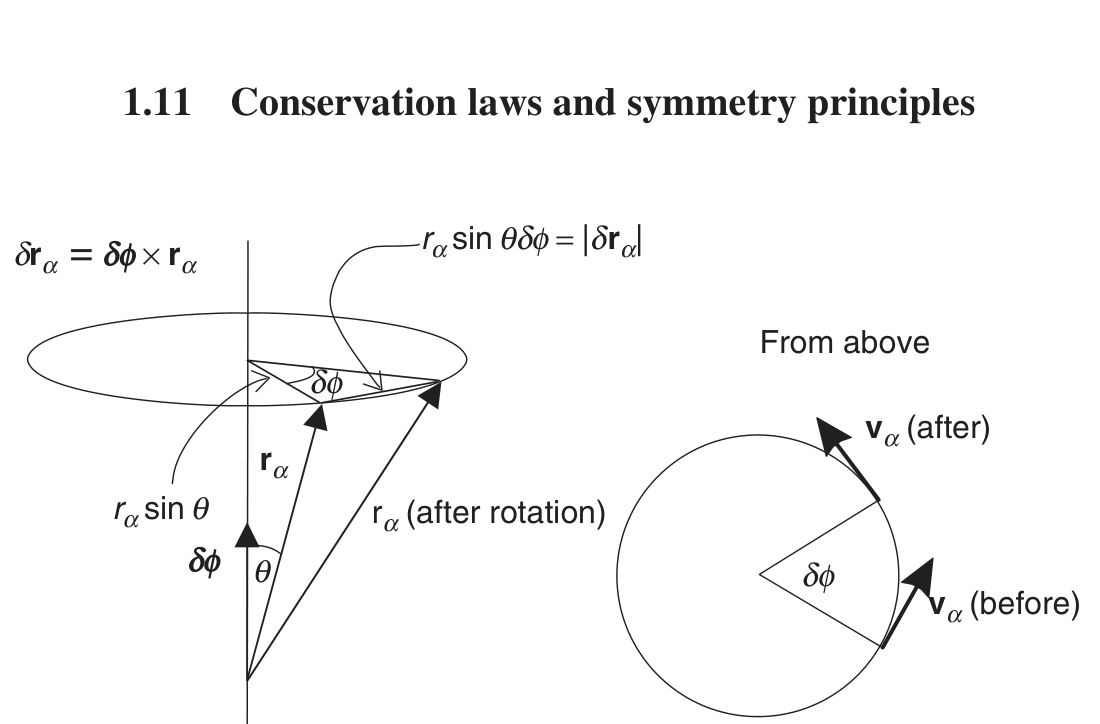
\includegraphics[width=0.55\linewidth]{../Figures/fig_1_10.png}
\caption{Figure 1.10}
\end{figure}

If the space is isotropic, the rotation will have no effect on the Lagrangian
so \textbackslash{}delta L = 0. That is,
0 = \textbackslash{}delta L =
\textbackslash{}alpha
\textbackslash{}partial L
\textbackslash{}partial r\textbackslash{}alpha
\textbackslash{}cdot  \textbackslash{}delta r\textbackslash{}alpha  + \textbackslash{}partial L
\textbackslash{}partial v\textbackslash{}alpha
\textbackslash{}cdot  \textbackslash{}delta v\textbackslash{}alpha

.
(Note that in this situation the velocities of the particles are not constant.)
Again, we use Lagrange's equation to replace \textbackslash{}partial L
\textbackslash{}partial r\textbackslash{}alpha  with d
dt
\textbackslash{}partial L
\textbackslash{}partial v\textbackslash{}alpha  =
dt p\textbackslash{}alpha  = $\textbackslash{}dot p$\textbackslash{}alpha
and write

\textbackslash{}alpha
$\textbackslash{}dot p$\textbackslash{}alpha  \textbackslash{}cdot  \textbackslash{}delta r\textbackslash{}alpha  + p\textbackslash{}alpha  \textbackslash{}cdot  \textbackslash{}delta v\textbackslash{}alpha

= 0.
From the figure, \textbar{}\textbackslash{}delta r\textbar{} = r sin \textbackslash{}theta \textbackslash{}delta \textbackslash{}phi . But since \textbackslash{}delta r is perpendicular to both r and
\textbackslash{}delta \textbackslash{}phi , we can write \textbackslash{}delta r = \textbackslash{}delta \textbackslash{}phi  \textbackslash{}times  r. Similarly, \textbackslash{}delta v = \textbackslash{}delta \textbackslash{}phi  \textbackslash{}times  v. Therefore,

\textbackslash{}alpha
$\textbackslash{}dot p$\textbackslash{}alpha  \textbackslash{}cdot  \textbackslash{}delta \textbackslash{}phi  \textbackslash{}times  r\textbackslash{}alpha  + p\textbackslash{}alpha  \textbackslash{}cdot  \textbackslash{}delta \textbackslash{}phi  \textbackslash{}times  v\textbackslash{}alpha

= 0.
Interchanging the dot and the cross we obtain

\textbackslash{}alpha
\textbackslash{}delta \textbackslash{}phi \textbackslash{}cdot

r\textbackslash{}alpha  \textbackslash{}times  $\textbackslash{}dot p$\textbackslash{}alpha  + $\textbackslash{}dot r$\textbackslash{}alpha  \textbackslash{}times  p\textbackslash{}alpha

= \textbackslash{}delta \textbackslash{}phi \textbackslash{}cdot
\textbackslash{}alpha
dt

r\textbackslash{}alpha  \textbackslash{}times  p\textbackslash{}alpha

= 0.

Consequently, since \textbackslash{}delta \textbackslash{}phi ̸ =0

\textbackslash{}alpha
dt (r\textbackslash{}alpha  \textbackslash{}times  p\textbackslash{}alpha ) = d
dt

\textbackslash{}alpha
r\textbackslash{}alpha  \textbackslash{}times  p\textbackslash{}alpha  = dL
dt = 0,
where L is the total angular momentum. That is, the isotropy of space leads
to the conservation of angular momentum. (Be careful not to confuse the total
vector angular momentum, L, with the Lagrangian L.)
\end{exercise}

\begin{exercise}
Exercise 1.22 Using the elementary mechanics approach, show that the
angular momentum of a system of particles is constant if no net external
torque acts on the system. Note that you must invoke Newton's third law
in the strong form.
1.11.4 The conservation of energy and the work function
Consider the kinetic energy of a single particle. In introductory physics we
learned the work--energy theorem, which states that the net work done on the
particle by external forces will result in an equal increase in the kinetic energy
of the particle. By definition, work is
W =

F \textbackslash{}cdot  ds.
Consequently, the increase in kinetic energy of a particle acted upon by a force
F as it goes from point 1 to point 2 is
T2 -T1 =
F \textbackslash{}cdot  ds.
If the force is conservative, the quantity F \textbackslash{}cdot  ds is the differential of a scalar
quantity denoted by U and called the ``work function.'' The concept of work
function has been replaced in modern terminology by potential energy (V )
defined as the negative of the work function.
V = -U.
This means that if the force is conservative it can be expressed in terms of the
gradient of a scalar function, thus
F = -\textbackslash{}nabla V.
Then the work energy theorem yields
T2 -T1 =
-\textbackslash{}nabla V \textbackslash{}cdot ds.

1.11
Conservation laws and symmetry principles
But \textbackslash{}nabla V \textbackslash{}cdot  ds = dV, so
T2 -T1 = -(V2 -V1),
or
T2 + V2 = T1 + V1.
This equation expresses the conservation of mechanical energy; it indicates
that there is a quantity that remains constant as the system is taken from one
configuration to another under the action of conservative forces. This quantity
is, of course, the total mechanical energy E = T + V.
The condition for a force to be conservative is that it is equal to the negative
gradient of a scalar function. This is equivalent to requiring that the curl of the
force be zero, i.e. \textbackslash{}nabla \textbackslash{}times  F = 0.
The preceding discussion of the conservation of energy was fairly elementary. We now consider energy from an advanced point of view and show that
the conservation of energy follows from the homogeneity of time.
In general, the derivative of the Lagrangian L = L(q, $\textbackslash{}dot q$, t) with respect to
time is
dt =
\textbackslash{}partial L
\textbackslash{}partial qi
dqi
dt +
\textbackslash{}partial L
\textbackslash{}partial $\textbackslash{}dot q$i
d $\textbackslash{}dot q$i
dt + \textbackslash{}partial L
\textbackslash{}partial t .
By Lagrange's equation, \textbackslash{}partial L
\textbackslash{}partial qi = d
dt
\textbackslash{}partial L
\textbackslash{}partial $\textbackslash{}dot q$i , so
dt =

$\textbackslash{}dot q$i
dt
\textbackslash{}partial L
\textbackslash{}partial $\textbackslash{}dot q$i

+ \textbackslash{}partial L
\textbackslash{}partial $\textbackslash{}dot q$i
d $\textbackslash{}dot q$i
dt

+ \textbackslash{}partial L
\textbackslash{}partial t .
But note that
dt

$\textbackslash{}dot q$i
\textbackslash{}partial L
\textbackslash{}partial $\textbackslash{}dot q$i
=
dt

$\textbackslash{}dot q$i
\textbackslash{}partial L
\textbackslash{}partial $\textbackslash{}dot q$i

=

$\textbackslash{}dot q$i
dt
\textbackslash{}partial L
\textbackslash{}partial $\textbackslash{}dot q$i

+ d $\textbackslash{}dot q$i
dt
\textbackslash{}partial L
\textbackslash{}partial $\textbackslash{}dot q$i

,
so the summation in the preceding equation can be replaced by d
dt

$\textbackslash{}dot q$i \textbackslash{}partial L
\textbackslash{}partial $\textbackslash{}dot q$i ,
and
dt = d
dt

$\textbackslash{}dot q$i
\textbackslash{}partial L
\textbackslash{}partial $\textbackslash{}dot q$i
+ \textbackslash{}partial L
\textbackslash{}partial t ,
or
\textbackslash{}partial L
\textbackslash{}partial t = d
dt

L -
$\textbackslash{}dot q$i
\textbackslash{}partial L
\textbackslash{}partial $\textbackslash{}dot q$i

.

We now introduce a new quantity called the energy function h that is
defined by
h = h(q, $\textbackslash{}dot q$, t) =
$\textbackslash{}dot q$i
\textbackslash{}partial L
\textbackslash{}partial $\textbackslash{}dot q$i
-L,
so that
\textbackslash{}partial L
\textbackslash{}partial t = -dh
dt .
Note that h depends on the generalized positions and the generalized velocities.
Let us assume temporal homogeneity so that time does not appear explicitly
in the Lagrangian. Then \textbackslash{}partial L
\textbackslash{}partial t = 0 and consequently
dt

L -
$\textbackslash{}dot q$i
\textbackslash{}partial L
\textbackslash{}partial $\textbackslash{}dot q$i

= -dh
dt = 0.
That is, the energy function is constant. But does this imply that the energy
(E = T + V ) is constant? To answer this question we note that the kinetic
energy has the general form
T = T0 + T1 + T2,
where T0 does not depend on velocities, T1 is a homogeneous function of the
first degree in velocities and T2 is a homogeneous function of second degree
in velocities.10 (In Cartesian coordinates, T0 and T1 are both zero, and T2 is
not only of second degree in velocities, but is actually a quadratic function of
velocities, i.e. it contains $\textbackslash{}dot x$2 but not $\textbackslash{}dot x$ $\textbackslash{}dot y$.)
Recall that a function f (x1, . . . , xn) is homogeneous of degree k if
f (\textbackslash{}alpha x1, \textbackslash{}alpha x2, . . . , \textbackslash{}alpha xn) = \textbackslash{}alpha kf (x1, . . . , xn).
Euler's theorem on homogeneous functions states that, if f ($\textbackslash{}xi$) is homogenous
of degree k, then

\textbackslash{}partial f
\textbackslash{}partial $\textbackslash{}xi$
= kf.
Since the kinetic energy has the general form T0 + T1 + T2, the Lagrangian
also has this form: L = L0 + L1 + L2. Then by Euler's theorem,
10 This can be proved by starting with the kinetic energy in Cartesian coordinates and then
using the transformation equations $\textbackslash{}xi$ = $\textbackslash{}xi$(q1, q2, . . . , qn, t), and the fact that
$\textbackslash{}dot x$i =
j
\textbackslash{}partial $\textbackslash{}xi$
\textbackslash{}partial qj $\textbackslash{}dot q$j + \textbackslash{}partial $\textbackslash{}xi$
\textbackslash{}partial t . See Problem 1.12 at the end of the chapter.

1.11
Conservation laws and symmetry principles

$\textbackslash{}dot q$i
\textbackslash{}partial L0
\textbackslash{}partial $\textbackslash{}dot q$i
= 0

$\textbackslash{}dot q$i
\textbackslash{}partial L1
\textbackslash{}partial $\textbackslash{}dot q$i
= L1

$\textbackslash{}dot q$i
\textbackslash{}partial L2
\textbackslash{}partial $\textbackslash{}dot q$i
= 2L2.
Therefore,

$\textbackslash{}dot q$i
\textbackslash{}partial L
\textbackslash{}partial $\textbackslash{}dot q$i
=
$\textbackslash{}dot q$i
\textbackslash{}partial (L0 + L1 + L2)
\textbackslash{}partial $\textbackslash{}dot q$i
= L1 + 2L2,
and

$\textbackslash{}dot q$i
\textbackslash{}partial L
\textbackslash{}partial $\textbackslash{}dot q$i
-L = (L1 + 2L2) -(L0 + L1 + L2) = L2 -L0.
If the transformation equations do not involve t explicitly, T = T2, that is, T
is a homogeneous function of second degree in the velocities. And if V does
not depend on velocities, L0 = -V. Then
h = T + V = E.
As long as these conditions are satisfied, the energy function is equal to the
total energy and the total energy is conserved.
If we replace \textbackslash{}partial L
\textbackslash{}partial $\textbackslash{}dot q$i by pi, the energy function is transformed into the Hamiltonian, which is a function of the generalized coordinates and the generalized
momenta:
H = H(q, p, t) =
$\textbackslash{}dot q$ipi -L.
The energy function and the Hamiltonian are essentially the same thing, but
they are expressed in terms of different variables, that is, h = h(q, $\textbackslash{}dot q$, t) and
H = H(q, p, t). (Whereas h depends on velocity, H depends on momentum.)
\end{exercise}

\begin{exercise}
Exercise 1.23 (a) Show that F = -y\textbackslash{}hat\{i\}+x\textbackslash{}hat\{j\} is not conservative. (b) Show
that F = y\textbackslash{}hat\{i\}+x\textbackslash{}hat\{j\} is conservative.
\end{exercise}

\begin{exercise}
Exercise 1.24 Show that F = 3x2y\textbackslash{}hat\{i\} + (x3 + 1)\textbackslash{}hat\{j\} + 9z2\textbackslash{}hat\{k\} is conservative.
\end{exercise}

\begin{exercise}
Exercise 1.25 Prove that the curl of a conservative force is zero.
\end{exercise}

\begin{exercise}
Exercise 1.26 Prove Euler's theorem. (Hint: Differentiate f (tx, ty, tz) =
tkf (x, y, z) with respect to t, then let t = 1.)

\end{exercise}

\begin{exercise}
Exercise 1.27 Show that z2 ln(x/y) is homogeneous of degree 2.
\end{exercise}

\begin{exercise}
Exercise 1.28 Show that
$\textbackslash{}dot q$i \textbackslash{}partial L2
\textbackslash{}partial $\textbackslash{}dot q$i = 2L2.
The virial theorem
The virial theorem states that for a bounded conservative system (such as a
planet going around a star) the average value of the kinetic energy is proportional to the average value of the potential energy. (For the planet/star we find
⟨T ⟩= -(1/2) ⟨V ⟩.) We now prove the theorem.
In Cartesian coordinates the kinetic energy is a homogenous quadratic function depending only on the velocities, so Euler's theorem yields

\textbackslash{}alpha
v\textbackslash{}alpha  \textbackslash{}cdot  \textbackslash{}partial T
\textbackslash{}partial v\textbackslash{}alpha
= 2T.
As long as the potential energy does not depend on velocities, the momentum
can be expressed as
p\textbackslash{}alpha  = \textbackslash{}partial T
\textbackslash{}partial v\textbackslash{}alpha
,
and hence
2T =
\textbackslash{}alpha
p\textbackslash{}alpha  \textbackslash{}cdot  v\textbackslash{}alpha  =
\textbackslash{}alpha
p\textbackslash{}alpha  \textbackslash{}cdot  dr\textbackslash{}alpha
dt .
But
dt

\textbackslash{}alpha
p\textbackslash{}alpha  \textbackslash{}cdot  r\textbackslash{}alpha  =
\textbackslash{}alpha
p\textbackslash{}alpha  \textbackslash{}cdot  dr\textbackslash{}alpha
dt +
\textbackslash{}alpha
dp\textbackslash{}alpha
dt \textbackslash{}cdot  r\textbackslash{}alpha .
Therefore
2T = d
dt

\textbackslash{}alpha
p\textbackslash{}alpha  \textbackslash{}cdot  r\textbackslash{}alpha  -
\textbackslash{}alpha
dp\textbackslash{}alpha
dt \textbackslash{}cdot  r\textbackslash{}alpha .
Now by Newton's second law, for a conservative system,
dp\textbackslash{}alpha
dt
= F\textbackslash{}alpha  = -\textbackslash{}partial V
\textbackslash{}partial r\textbackslash{}alpha
,
so
2T = d
dt

\textbackslash{}alpha
p\textbackslash{}alpha  \textbackslash{}cdot  r\textbackslash{}alpha  +
\textbackslash{}alpha
\textbackslash{}partial V
\textbackslash{}partial r\textbackslash{}alpha
\textbackslash{}cdot  r\textbackslash{}alpha .
Let us evaluate the average value of all the terms in this equation:
⟨2T ⟩=
d
dt

\textbackslash{}alpha
p\textbackslash{}alpha  \textbackslash{}cdot  r\textbackslash{}alpha

+

\textbackslash{}alpha
r\textbackslash{}alpha  \textbackslash{}cdot  \textbackslash{}partial V
\textbackslash{}partial r\textbackslash{}alpha

.

1.12
Problems
Recall that the time average of a function f (t) is
⟨f (t)⟩= lim
\textbackslash{}tau \textbackslash{}to \textbackslash{}infty
\textbackslash{}tau
\textbackslash{}tau
f (t)dt,
so d
dt

\textbackslash{}alpha
p\textbackslash{}alpha  \textbackslash{}cdot  r\textbackslash{}alpha

= lim
\textbackslash{}tau \textbackslash{}to \textbackslash{}infty
\textbackslash{}tau
\textbackslash{}tau
dt

\textbackslash{}alpha
p\textbackslash{}alpha  \textbackslash{}cdot  r\textbackslash{}alpha dt = lim
\textbackslash{}tau \textbackslash{}to \textbackslash{}infty
\textbackslash{}tau
\textbackslash{}tau

\textbackslash{}alpha
p\textbackslash{}alpha  \textbackslash{}cdot  r\textbackslash{}alpha

= lim
\textbackslash{}tau \textbackslash{}to \textbackslash{}infty
\textbackslash{}tau

\textbackslash{}alpha
p\textbackslash{}alpha  \textbackslash{}cdot  r\textbackslash{}alpha
\textbackslash{}tau
= lim
\textbackslash{}tau \textbackslash{}to \textbackslash{}infty

\textbackslash{}alpha
p\textbackslash{}alpha  \textbackslash{}cdot  r\textbackslash{}alpha

\textbackslash{}tau
-
\textbackslash{}alpha
p\textbackslash{}alpha  \textbackslash{}cdot  r\textbackslash{}alpha

\textbackslash{}tau
= 0,
where we assumed that
\textbackslash{}alpha
p\textbackslash{}alpha  \textbackslash{}cdot  r\textbackslash{}alpha  remains finite at all times. In other words,
we are assuming the motion is bounded, so the numerator is finite but the
denominator goes to infinity.
We are left with
2 ⟨T ⟩=

\textbackslash{}alpha
r\textbackslash{}alpha  \textbackslash{}cdot  \textbackslash{}partial V
\textbackslash{}partial r\textbackslash{}alpha

.
If the potential energy is a homogeneous function of position of degree k, then
by Euler's theorem the right-hand side is kV, and
2 ⟨T ⟩= k ⟨V ⟩.
Thus, for example, for a particle of mass m in a gravitational field,
V = -GMm
r
so k = -1 and
2 ⟨T ⟩= -⟨V ⟩.
Since E = T + V, we see that ⟨E⟩= -⟨T ⟩, indicating that the total energy is
negative, and that the magnitude of the average kinetic energy is one half the
magnitude of the average potential energy.
As another example, consider a mass on a spring. The potential energy is
V = (1/2)Kx2 so k = 2 and 2 ⟨T ⟩= 2 ⟨V ⟩, that is, ⟨T ⟩= ⟨V ⟩.
\end{exercise}

\section*{1.12  Problems}

\section*{1.1  There is a story about a physicist who got a traffic ticket for running a red}

light. Being a clever person the physicist proved to the judge that it was
neither possible to stop nor to continue without either running the light
or breaking the speed limit. In this problem we determine if the story is
credible or is just a figment of the imagination of an overworked graduate

student. Assume the physicist is driving a car at a constant speed v0, equal
to the speed limit. The car is a distance d from an intersection when the
light changes from green to yellow. The physicist has a reaction time \textbackslash{}tau  and
the car brakes with a constant deceleration ac. The light remains yellow for
a time ty. Determine the conditions such that the car can neither stop nor
continue at v0 without running the red light. Also, using realistic values
for \textbackslash{}tau , ty, ac and v0 determine whether or not this situation could actually
arise. (Solve using simple kinematic relations.)
\section*{1.2  A cylinder of mass M and radius R is set on end on a table at a distance L}

\begin{figure}[h]
\centering
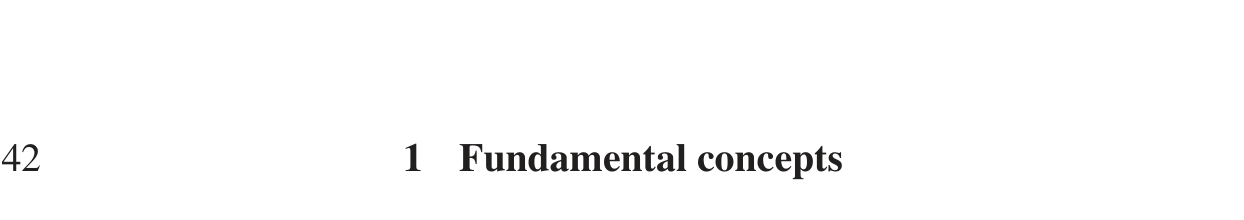
\includegraphics[width=0.55\linewidth]{../Figures/fig_1_11.png}
\caption{Figure 1.11}
\end{figure}

the cylinder. The free end of the string passes over a frictionless pulley and
hangs off the edge of the table. A weight of mass m is attached to the free
end of the string. Determine the time required for the spool to reach the
edge of the table.
A cylinder on a frictionless table.
1.3 A string passes over a massless pulley. Each end is wound around a vertical
\begin{figure}[h]
\centering
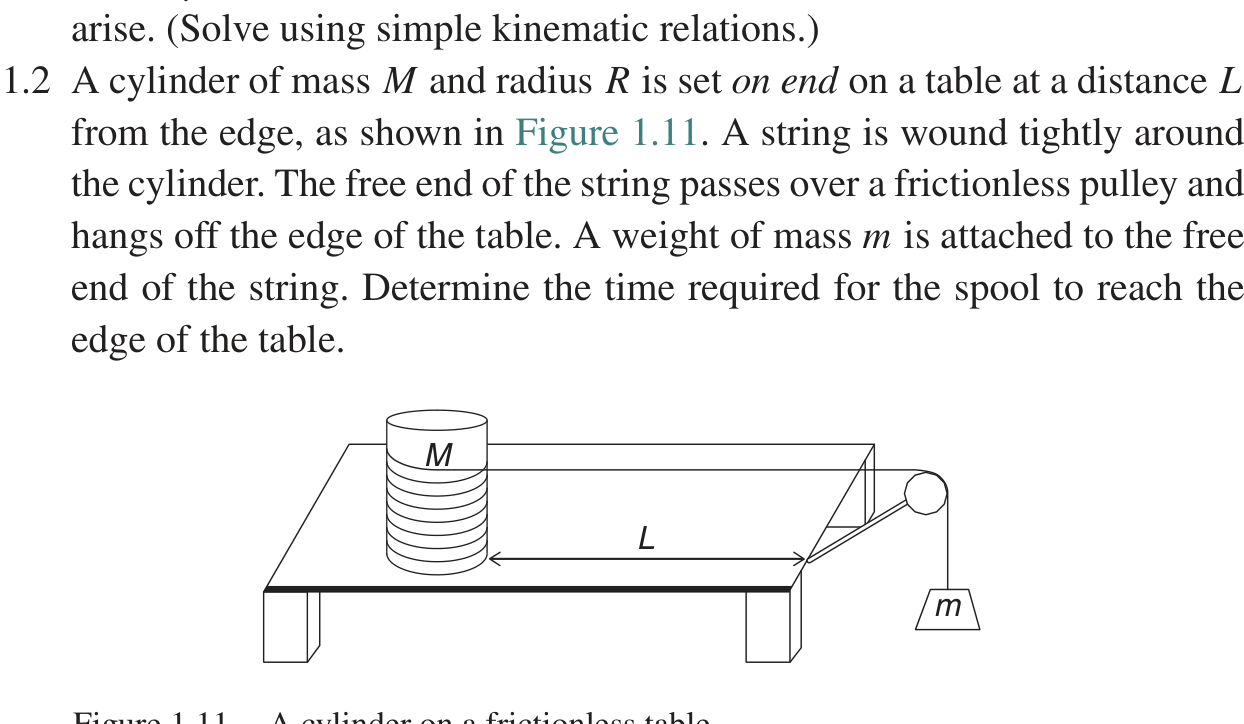
\includegraphics[width=0.55\linewidth]{../Figures/fig_1_12.png}
\caption{Figure 1.12}
\end{figure}

string, but if one hoop is much more massive than the other, it can cause
the lighter hoop to rise. The hoops have masses M1 and M2 and radii R1
and R2. Show that the tension in the string is \textbackslash{}tau  = gM1M2 (M1 + M2)-1 .
M1
M2
Two hoops hang from a pulley. The string unwinds as the hoops
descend.

1.12
Problems
1.4 The transformation equations for the bipolar coordinates \textbackslash{}eta  and \textbackslash{}zeta  are
x =
a sinh \textbackslash{}eta
cosh \textbackslash{}eta  -cos \textbackslash{}zeta  ,
y =
a sin \textbackslash{}zeta
cosh \textbackslash{}eta  -cos \textbackslash{}zeta  .
(a) Show that the inverse transformation exists. (b) Obtain expressions for
\textbackslash{}eta  and \textbackslash{}zeta  in terms of x and y.
\section*{1.5  A disk of mass m and radius a rolls down a perfectly rough inclined plane}

of angle \textbackslash{}alpha . Determine the equations of motion and the constraints acting
on the disk.
\section*{1.6  A pendulum of length l and mass m is mounted on a cart of mass M that}

is free to roll along a track. There is no friction. Write the Lagrangian for
the pendulum/cart system.
\section*{1.7  Starting with the definition}

T = 1
N
i=1

$\textbackslash{}dot x$2
i + $\textbackslash{}dot y$2
i + $\textbackslash{}dot z$2

and the transformation equations, show that
T =
3N

j=1
3N

k=1
2Ajk $\textbackslash{}dot q$j $\textbackslash{}dot q$k +
3N

j=1
Bj $\textbackslash{}dot q$j + T0,
where
Ajk =
N
i=1
\textbackslash{}partial $\textbackslash{}xi$
\textbackslash{}partial qj
\textbackslash{}partial $\textbackslash{}xi$
\textbackslash{}partial qk
+ \textbackslash{}partial yi
\textbackslash{}partial qj
\textbackslash{}partial yi
\textbackslash{}partial qk
+ \textbackslash{}partial zi
\textbackslash{}partial qj
\textbackslash{}partial zi
\textbackslash{}partial qk

,
Bj =
N
i=1
\textbackslash{}partial $\textbackslash{}xi$
\textbackslash{}partial qj
\textbackslash{}partial $\textbackslash{}xi$
\textbackslash{}partial t + \textbackslash{}partial yi
\textbackslash{}partial qj
\textbackslash{}partial yi
\textbackslash{}partial t + \textbackslash{}partial zi
\textbackslash{}partial qj
\textbackslash{}partial zi
\textbackslash{}partial t

,
T0 =
N
i=1
2mi
\textbackslash{}partial $\textbackslash{}xi$
\textbackslash{}partial t
+
\textbackslash{}partial yi
\textbackslash{}partial t
+
\textbackslash{}partial zi
\textbackslash{}partial t
.

\section*{2.1  Introduction}

The calculus of variations is a branch of mathematics which considers extremal
problems; it yields techniques for determining when a particular definite integral will be a maximum or a minimum (or, more generally, the conditions for
the integral to be ``stationary''). The calculus of variations answers questions
such as the following.
• What is the path that gives the shortest distance between two points in a
plane? (A straight line.)
• What is the path that gives the shortest distance between two points on a
sphere? (A geodesic or ``great circle.'')
• What is the shape of the curve of given length that encloses the greatest
area? (A circle.)
• What is the shape of the region of space that encloses the greatest volume
for a given surface area? (A sphere.)
The technique of the calculus of variations is to formulate the problem in
terms of a definite integral, then to determine the conditions under which the
integral will be maximized (or minimized). For example, consider two points
(P1 and P2) in the x--y plane. These can be connected by an infinite number
of paths, each described by a function of the form y = y(x). Suppose we
wanted to determine the equation y = y(x) for the curve giving the shortest
path between P1 and P2. To do so we note that the distance between the two
end points is given by the definite integral
I =
P2
P1
ds,
where ds is an infinitesimal distance along the curve. Our task is to determine
the function y = y(x) such that I is minimized.